\documentclass[12pt]{article}

\usepackage{fullpage}
\usepackage{epsfig}
\usepackage{longtable}
\usepackage{fontenc}
\usepackage{graphicx}
\usepackage{times}
\usepackage{rotating}
\usepackage{psfrag}
\usepackage{graphics}
\usepackage{lscape}

\bibliographystyle{input/prsty.bst}

\makeatletter
\renewcommand{\thefootnote}{\fnsymbol{footnote}}
\newcommand{\boldsymbol}[1]{\mbox{\boldmath $#1$}}
\makeatother

\def\total_days{39.8}
\def\production_days{28}
\def\overhead_days{11.8}

\def\QMIN{1.5}
\def\QMAX{3.6}
\def\XMIN{0.30}
\def\XMAX{0.50}
\def\WMIN{1.8}

\def\PZ{35}     % Vector target polarization
\def\PF{0.55 }   % Packing Factor
\def\DF{0.30 }   % Dilution Factor
\def\TARGET{ND$_3$ }
\def\CURRENT{115 } % nanoAmps

\def\be{\begin{eqnarray*}}
\def\ee{\end{eqnarray*}}
\def\bn{\begin{eqnarray}}
\def\en{\end{eqnarray}}
\def\nn{\nonumber}

\def\ks{\vspace{1.4cm}\\}
\def\ls{\vspace{0.1cm}}

\def\n{\large}




%%%%%%%%%%%%%%%

\begin{document}

\pagestyle{empty}
 
\begin{center}
 \LARGE{
  The Deuteron Tensor Structure Function $b_1$
 }
\end{center}
%
\hrule \vspace{.05cm}\hrule
%
\begin{center}
A Proposal to Jefferson Lab PAC-38

(Update to LOI-11-003)

\vspace{1.5cm}

\setcounter{footnote}{1}
%
{\n J.-P. Chen (co-spokesperson),~~ P. Solvignon (co-spokesperson),\\
K. Allada,~~ A. Camsonne,~~ A. Deur,~~ D. Gaskell,\\
M. Jones,~~C. Keith,~~J. Pierce,~~S. Wood,~~J. Zhang}\\
\ls
{\normalsize\it{Thomas Jefferson National Accelerator Facility, Newport News, VA 23606}}
\ks
%
%
{\n N. Kalantarians (co-spokesperson),~~ O. Rondon (co-spokesperson)\\
Donald  Crabb,~~ Donal B. Day,~~ Hovhannes Baghdasaryan,~~ Charles Hanretty\\
Richard Lindgren,~~Blaine Norum,~~ Zhihong Ye,~~ X. Zheng}\\
\ls
{\normalsize\it{University of Virginia, Charlottesville, VA 22903}}
\ks
%
%
{\n K. Slifer\footnotemark (co-spokesperson),~~A. Atkins,~~ T. Badman,\\
J. Calarco,~~J. Dawson,~~ J. Maxwell,~~ S. Phillips,~~ R. Zielinski}\\
\ls
{\normalsize\it{University of New Hampshire, Durham, NH 03861}}
\ks
%
%
{\n J. Dunne,~~D. Dutta} \\
\ls
{\normalsize\it{Mississippi State University, %Department of Physics and Astronomy, 
Mississippi State, MS 39762}}
\ks
{\n G. Ron} \\
\ls
{\normalsize\it{Hebrew University of Jerusalem, Jerusalem
}}
\ks
%
{\n W. Bertozzi,~~ S. Gilad, ~~J. Huang\\
A. Kelleher,~~ V. Sulkosky} \\
\ls
{\normalsize\it{Massachusetts Institute of Technology, Cambridge, MA 02139
}}
\ks
%
%
{\n K. Adhikari} \\
\ls
{\normalsize\it{Old Dominion University, Norfolk, VA 23529}}
\ks
{\n R. Gilman} \\
\ls
{\normalsize\it{ Rutgers, The State University of New Jersey, Piscataway, NJ 08854}}
\ks
%
{\n Seonho Choi,~~ Hoyoung Kang,~~ Hyekoo Kang,~~ Yoomin Oh} \\
\ls
{\normalsize\it{ Seoul National University, Seoul 151-747 Korea}}
\ks
%
%{\n Alessandro Bacchetta}\\
%\ls
%{\normalsize\it{ Dipartimento di Fisica Nucleare e Teorica
%       Universitą di Pavia, via Bassi 6
%       27100 Pavia, Italy}}
%\ks
{\n H.~P.~ Cheng,~~ H.~J.~ Lu,~~ X.~H.~ Yan }\\
\ls
{\normalsize\it{Institute of Applied Physics, Huangshan University, Huangshan, P. R. China}}
\ks
{\n Y.~X.~Ye,~~ P.~J.~Zhu}\\
\ls
{\normalsize\it{
University of Science and Technology of China, Hefei 230026, P. R. China}}
\ks
%
{\n B.~T.~Hu,~~Y. Zhang}\\
\ls
{\normalsize\it{Lanzhou University, Lanzhou, P. R. China.}}
\ks
%
{\n Abdellah Ahmidouch}\\
\ls
{\normalsize\it{
Department of Physics, North Carolina A \& T State University, Greensboro, NC 27401}}
\ks
{\n Caroline Riedl}\\
\ls
{\normalsize\it{DESY, Notkestrasse 85, 22603 Hamburg, Germany}}
\ks
%
\end{center}


\footnotetext{Contact person}


\newpage

\begin{abstract}
  The EMC experiment revealed that only a small fraction
of the nucleon spin is carried by quarks.
Two decades later, the spin crisis remains an open issue. 
Quark orbital angular momentum is now considered to be one of the principal 
contributions in generating the nucleon spin, but a precise determination of this
critical piece has remained elusive. The leading twist tensor structure function
$b_1$ of spin-1 hadrons 
can provide 
new insight into this puzzle, since it is directly related to effects arising from 
orbital angular momentum, which differ from the case in a spin-1/2 target.
%:  $b_1$ vanishes for the case of the deuteron constituents in a relative S state.  
For this reason, it provides a unique tool to study partonic effects, while also being sensitive to 
%cumulative nuclear properties, such as the EMC effect and other in-medium modifications to nucleon substructure.
coherent nuclear properties in the simplest nuclear system.

%Inclusive scattering from a spin-1 target is described by     
%eight structure functions. Four of these, the so-called tensor structure functions,
%do not exist in the case of a spin-1/2 target.


%Depending on the choice of Bjorken variable $x$, two separate phenomena can be explored via measurement
%of $b_1$. 
At low $x$, shadowing effects are expected to dominate $b_1$, 
while at larger values, $b_1$ provides a clean probe of exotic QCD effects, such as
hidden color due to 6-quark configuration. Since the 
%D-state contribution to the 
deuteron wave function is relatively well known, any novel effects are expected to be
readily observable.  All available models  predict a small or vanishing value of $b_1$ at moderate $x$.  However, the
first pioneer measurement of $b_1$ at HERMES revealed a crossover to an anomolously large negative value in the region $0.2 <x<0.5$, albeit with relatively large experimental uncertainty.  

We will perform an inclusive measurement of the deuteron polarized cross sections in the
region $\XMIN<x<\XMAX$, for $\QMIN<Q^2<\QMAX$ GeV$^2$.
With \production_days days of 11 GeV incident beam,  we can determine $b_1$ with sufficient 
precision to discriminate between conventional nuclear models, and the more exotic behaviour
which is hinted at by the HERMES data.
The UVa solid polarized \TARGET target will be used, along with the 
Hall C spectrometers, and an unpolarized  \CURRENT nA beam.
An additional \overhead_days days will be needed for overhead.
This measurement  will provide access to the tensor quark polarization, and allow a test of the 
Close-Kumano sum rule, which vanishes in the absence of tensor polarization in the quark 
sea. 
Until now, tensor structure has been largely unexplored, so the study 
of these quantities holds the potential of initiating a new field of spin physics at 
Jefferson Lab.


%fundamental quantities $\delta_{\dagger}q$ and $\delta_{\dagger}\overline{q}$






\end{abstract}

\newpage

\section*{Foreword}

This proposal follows the letter of intent LOI-11-003 which was submitted to PAC 37.  For convenience we reproduce the draft PAC report comments below.  We note that we plan to use Hall C's HMS/SHMS spectrometers, an option that we briefly explored in the appendix of the LOI. We have signficantly revised our experimental method, as discussed in Sec.~\ref{EXP},  which now makes the Hall C option compelling.   ND$_3$ has been selected as the target material instead of LiD in order to simplify the analysis, and to take advantage of the extensive experience using ND$_3$ within the collaboration and in the JLab Target group.  
We have also expanded our discussion in Sec.~\ref{PREDB1X} of the 
expected behaviour of $b_1(x)$, in order to strengthen the justification for measuring in
the region $\XMIN <x<\XMAX$, where most models predict very small or vanishing values for $b_1(x)$, in contrast to the HERMES data.


\vspace{1cm}
{\it
\noindent
{\bf LOI-11-003} ``The Deuteron Tensor Structure Function b1''

\vspace{0.5cm}
\noindent
{\bf Motivation}: The collaboration proposes to measure the deuteron tensor structure function b1 by measuring deep inelastic scattering from a tensor polarized deuterium. This structure function would be zero for a deuteron with constituents in a relative s-wave. The structure function b1 can be compared with conventional calculations of quark distribution functions convoluted with nucleon momentum distributions in the deuteron including the d-state admixture. Departures from such approach, as hinted at in pioneering data at HERMES, is conjectured to be sensitive to orbital angular momentum effects.

\vspace{1cm}
\noindent
{\bf Measurement and Feasibility}: The letter of intent proposes such experiment in Hall A using an 11 GeV beam and the SoLID spectrometer. The polarized target proposed is a $^6$LiD target. The rates in the proposal only assume tensor polarizations that have been demonstrated previously. The projected precision on the tensor structure function using SoLID is compelling to improve on the HERMES measurement at small x and extend it into the large x region. The proposed measurement will allow to map out the qualitative behavior of b1, which will serve as a benchmark for theoretical interpretations. In the appendix to the LOI, a feasibility study has also been performed for a measurement in Hall C using the HMS/SHMS spectrometers. Given the projected precision obtained, such measurement using HMS/SHMS does not seem to be compelling at this stage.


\vspace{1cm}\noindent
{\bf Issues}: The main issue is on the theoretical interpretation of such experiment. The authors are urged to consult some theorists to provide at least some qualitative behavior of b1 when making their physics case for a proposal.


\vspace{1cm}\noindent
{\bf Recommendation}: The PAC encourages the submission of a fully developed proposal that addresses the issue raised above.
}



\clearpage


\tableofcontents


\pagestyle{plain}

\clearpage

\section{Background and Motivation}
The deuteron is the simplest nuclear system, and in many ways it is as important to understanding bound states in QCD as the hydrogen atom was to understanding bound systems in QED.  Unlike it's atomic analogue, our understanding of the deuteron remains unsatisfying both experimentally and theoretically.  
%At low energy, one pion exchange provides a good description of the nucleon-nucleon interaction, whereas at high energies, partonic degrees of freedom are relevant.  At intermediate energies, no coherent description yet exists.  
A deeper understanding of the deuteron's tensor structure will help to clarify how the gross properties of the nucleus arise from the 
underlying partons.  This provides novel information about
nuclear structure, quark angular momentum, and the polarization of the quark sea  that is not accessible in spin-1/2 targets.  


A measurement of the tensor structure function $b_1$ is of considerable interest since it provides a clear measure of possible exotic effects in nuclei, i.e. the extent to which the nuclear ground state deviates from being a composite of nucleons only~\cite{Khan:1991qk}.
Jefferson Lab is the ideal place to investigate 
tensor structure in a deuteron target 
at intermediate and large $x$.  We describe such a measurement in this proposal.

\subsection{Tensor Structure of the Deuteron}
 %\subsubsection*{Tensor Polarization}
When a  spin 1 system such as the deuteron is subjected to a magnetic field along the z-axis, the
Zeeman interaction gives rise to three magnetic sublevels $I_z = +1,0,-1$ with
population fractions $p_+,p_-, p_0$, respectively.
%\footnote{i.e. $p_+ + p_- +p_0=1$.}.
These populations are described by
both a vector  polarization,
%
\begin{eqnarray}
\nonumber
P_z &=&\langle I_z/I\rangle \\
    &=&(p_+ - p_0) + (p_0-p_+) = p_+ - p_-
\end{eqnarray}
and a tensor polarization~\cite{Meyer:1985dta}:
\begin{eqnarray}
\nonumber
P_{zz} &=& \langle 3 I_z^2 - I(I+1)\rangle/I^2   \\
&=&(p_+ - p_0) - (p_0-p_-) = 1 - 3 p_0
\end{eqnarray}
%
which are subject to the overall normalization $p_+ + p_- + p_0 = 1$.

Fig.~\ref{fig:deuteron} graphically demonstrates the dependence of the two nucleon distribution on the spin projection.  If the two nucleons are in a relative $m=0$ state, the surface of constant density is toroidal, while if they are in the $m=\pm 1$ state, the surface has a dumbbell shape.

\begin{figure}
\centering
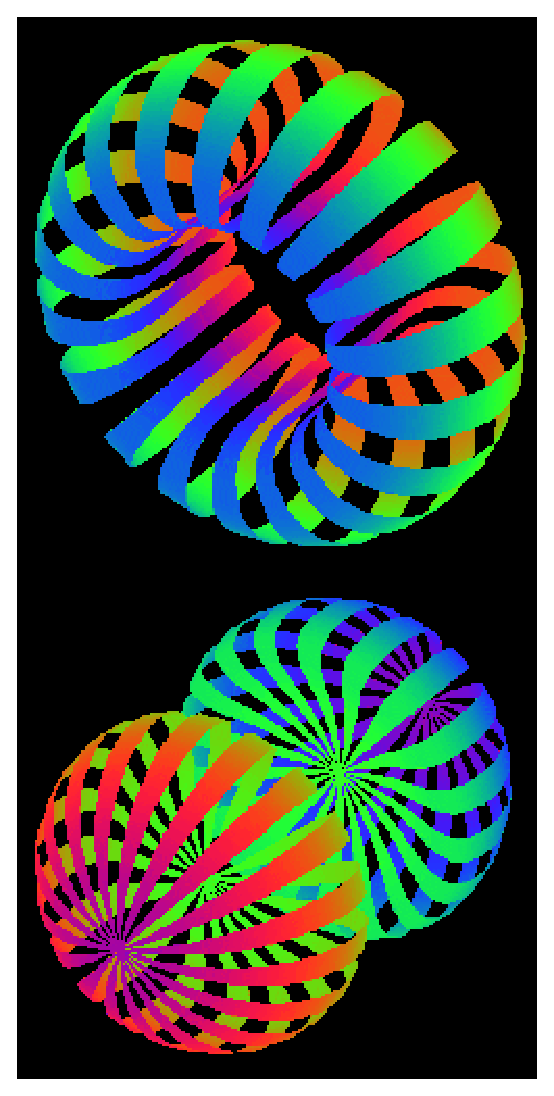
\includegraphics[width=0.3\textwidth,angle=90]{figs/pic-v10-st16-1.eps}
\caption{\label{fig:deuteron}
Nucleon densities of the deuteron in its two spin projections, $I_z=\pm 1$ and $I_z=0$, respectively.
{\it Reproduced from~\cite{Carlson:1997qn,Forest:1996kp}}.
}
\end{figure}

In the case of deuteron spins in thermal equilibrium with the solid lattice, and neglecting the small quadrupole interaction~\cite{Meyer:1985dta}, the tensor polarization is related to  the vector polarization via:
\begin{eqnarray}
\label{TENSORVECTOR}
P_{zz}= 2 - \sqrt{4-3 P_z^2}
\end{eqnarray}
The maximum absolute value of $P_{zz}=-2$  occurs only for vanishing populations in the $m=\pm 1$ states.
If, on the other hand, only the $m=1$ or $m=-1$ state are occupied, the vector polarization reaches its maximum value of $+1$, and $P_{zz}=+1$.  

\subsection{Deep Inelastic Scattering from Spin-1 Targets}
 %In this case, the familiar structure functions  $F_1$, $F_2$, $g_1$, and $g_2$ which describe
%inclusive scattering of electrons from spin-1/2 targets, must be supplemented for a spin-1 system
%by four additional structure functions : $b_1$, $b_2$, $b_3$, and $\Delta$.
%
%
%The tensor structure function $b_1$, ( which is leading-twist like  $F_1$ and $g_1$), is quite
%interesting, in that it presents a simple gauge of nuclear effects: $b_1$ would vanish if the
%deuteron was simply a proton and neutron in a relative S state.
%
%Nuclear effects/EMC effect
%%When spin physics joins naturally the nuclear effects area and model independent
%%nuclear effects extraction compared to polarized EMC effect.
%
%Exotic components.
%
%The Hermes collaboration  made a first measurement~\cite{Airapetian:2005cb} of
%$b_1$ and found significantly non-zero results.
%Beyond providing insight into nuclear structure, this has the potential to impact $g_1^n$ and
%$g_2^n$ extractions, where $b_1$ has traditionally been ignored when the neutron is extracted
%from deuteron data.
%

Four independent  helicity amplitudes are
sufficient to describe virtual Compton scattering from a spin-1/2 target, after requiring parity
and time reversal invariance.  This number doubles  for
a spin-1 target, as the spin can be in three states (+, 0, -). 
This gives rise to a tensor structure which was first discussed for the deuteron for the real photon case
by Pais~\cite{Pais:1967zz}, %in 1967 
and later in the virtual photon case, by Frankfurt and
Strikman~\cite{Frankfurt:1983qs}. %In 1988, 
Hoodbhoy, Jaffe and Manohar~\cite{Hoodbhoy:1988am}
introduced the notation which we now follow, whereby the tensor structure is described
by the four functions $b_1$, $b_2$, $b_3$ and $b_4$.
To summarize, the hadronic tensor can be decomposed as:
%
\begin{eqnarray}
W_{\mu\nu} &=& - F_1 g_{\mu\nu} + F_2 \frac{P_{\mu} P{\nu}}{\nu} \nonumber \\
          & & - b_1 r_{\mu\nu} + \frac{1}{6} b_2 (s_{\mu\nu} + t_{\mu\nu} + u_{\mu\nu}) \nonumber \\
          & & + \frac{1}{2} b_3 (s_{\mu\nu} - u_{\mu\nu}) + \frac{1}{2} b_4 (s_{\mu\nu} - t_{\mu\nu}) \nonumber \\
          & & + i \frac{g_1}{\nu} \epsilon_{\mu\nu\lambda\sigma} q^{\lambda} s^{\sigma} 
              + i \frac{g_2}{\nu^2} \epsilon_{\mu\nu\lambda\sigma} q^{\lambda} (p \cdot qs^{\sigma}  
              - s \cdot qp^{\sigma})
\label{had-tensor}
\end{eqnarray}
%
where the purely kinematic expressions  $r_{\mu\nu}$, $s_{\mu\nu}$, $t_{\mu\nu}$ and $u_{\mu\nu}$ can be 
found in~\cite{Hoodbhoy:1988am}. The terms are all proportional to the 
polarization of the target $E$. The spin-1 structure functions $F_1$, $F_2$, $g_1$ and 
$g_2$ have the same expressions and are measured the same way as for a spin-1/2 
target. The spin-dependent structure functions $b_1$, $b_2$, $b_3$, $b_4$ are 
symmetric under $\mu\leftrightarrow\nu$ and $E\leftrightarrow E^*$ and therefore can 
be isolated from $F_1$ and $g_1$ by unpolarized beam scattering from a polarized 
spin-1 target.


%\subsubsection{Existing Data}
% \label{B1DATASECTION}
%\begin{figure}
%\begin{center}
%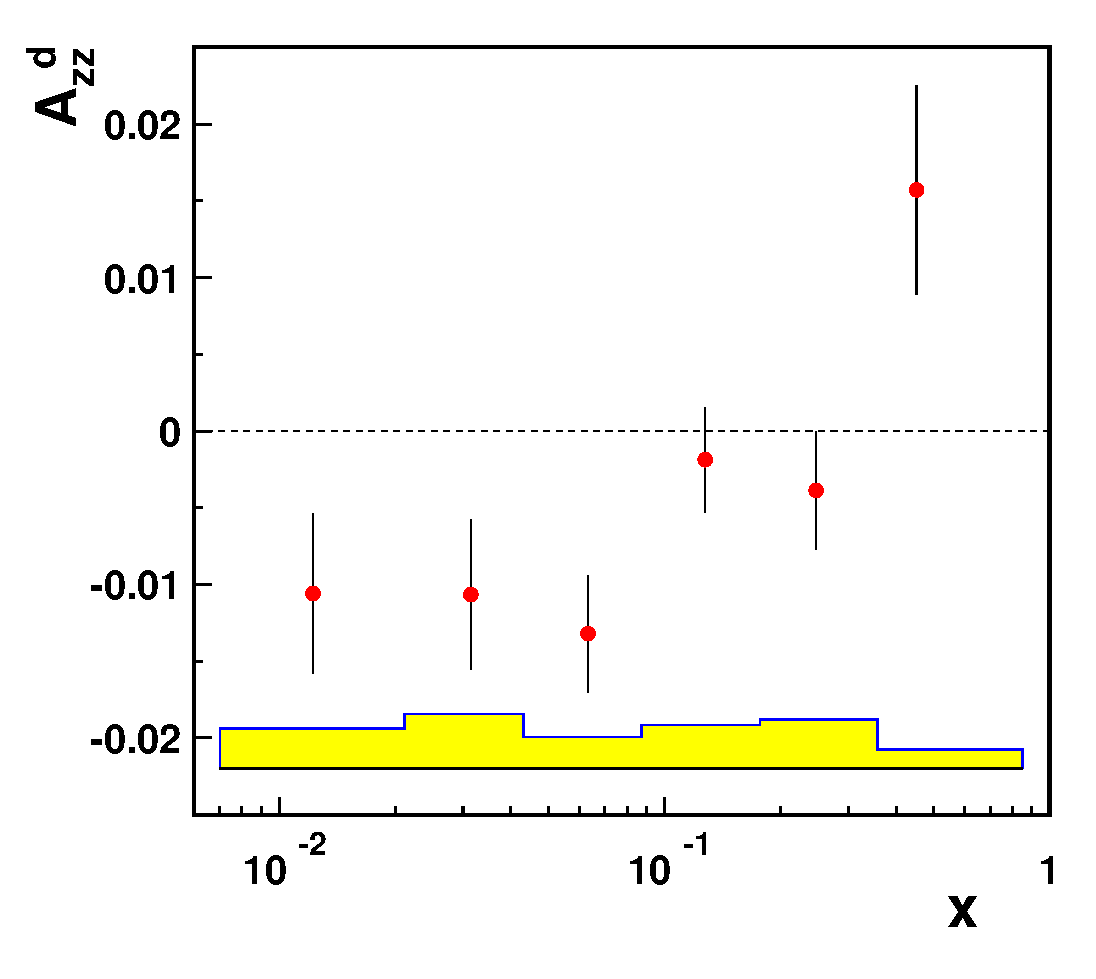
\includegraphics[angle=0,width=0.45\textwidth]{figs/azzfinal.eps}
%
%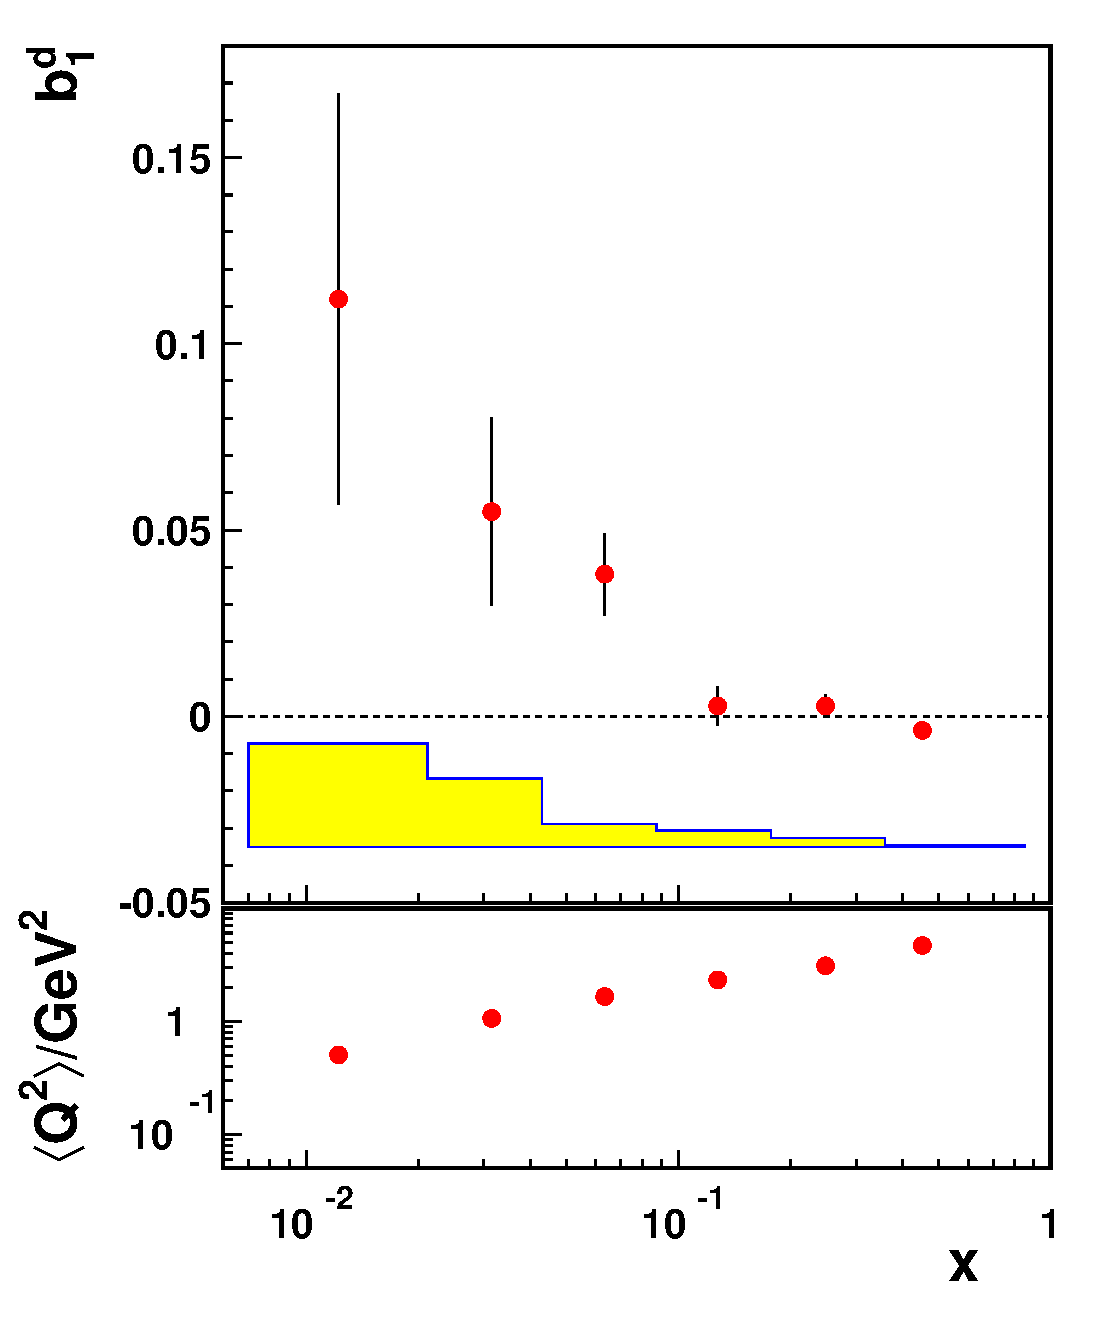
\includegraphics[angle=0,width=0.47\textwidth]{figs/b1final.eps}
%\caption{\label{HERMES_AZZ} {\bf Top:} HERMES measurement of the inclusive tensor asymmetry A$_{zz}$ of the deuteron.  
%{\bf Bottom:} HERMES measurement of the inclusive tensor structure function b$_1^d$ and the average $Q^2$ for each x-bin.  The error bands displays the total systematic uncertainty.
%{\it Reproduced from~\cite{Riedl:2005jq}.}}
%\end{center}\end{figure}

\begin{figure}
\begin{center}
\includegraphics[angle=0,width=0.45\textwidth]{figs/1.eps}
\hspace{0.5cm}
\includegraphics[angle=0,width=0.45\textwidth]{figs/2.eps}
\vspace{3cm}

\includegraphics[angle=0,width=0.45\textwidth]{figs/3.eps}
\caption{\label{HERMES_AZZ} {\bf Top}: HERMES~\cite{Riedl:2005jq} measurement of the inclusive tensor asymmetry A$_{zz}(x)$ and $xb_1(x)$ of the deuteron. {\bf Bottom} : The tensor structure function $b_1(x)$ without $x$-weighting, which reveals a steep rise as $x\to 0$. 
}
\end{center}\end{figure}

%\begin{figure}
%\begin{center}
%\includegraphics[angle=0,width=0.47\textwidth]{figs/2.eps}
%\caption{\label{HERMES_AZZ2} 
%HERMES~\cite{Riedl:2005jq} measurement of the inclusive tensor structure function b$_1^d$.  
%}
%\end{center}\end{figure}



%\begin{figure}
%\begin{center}
%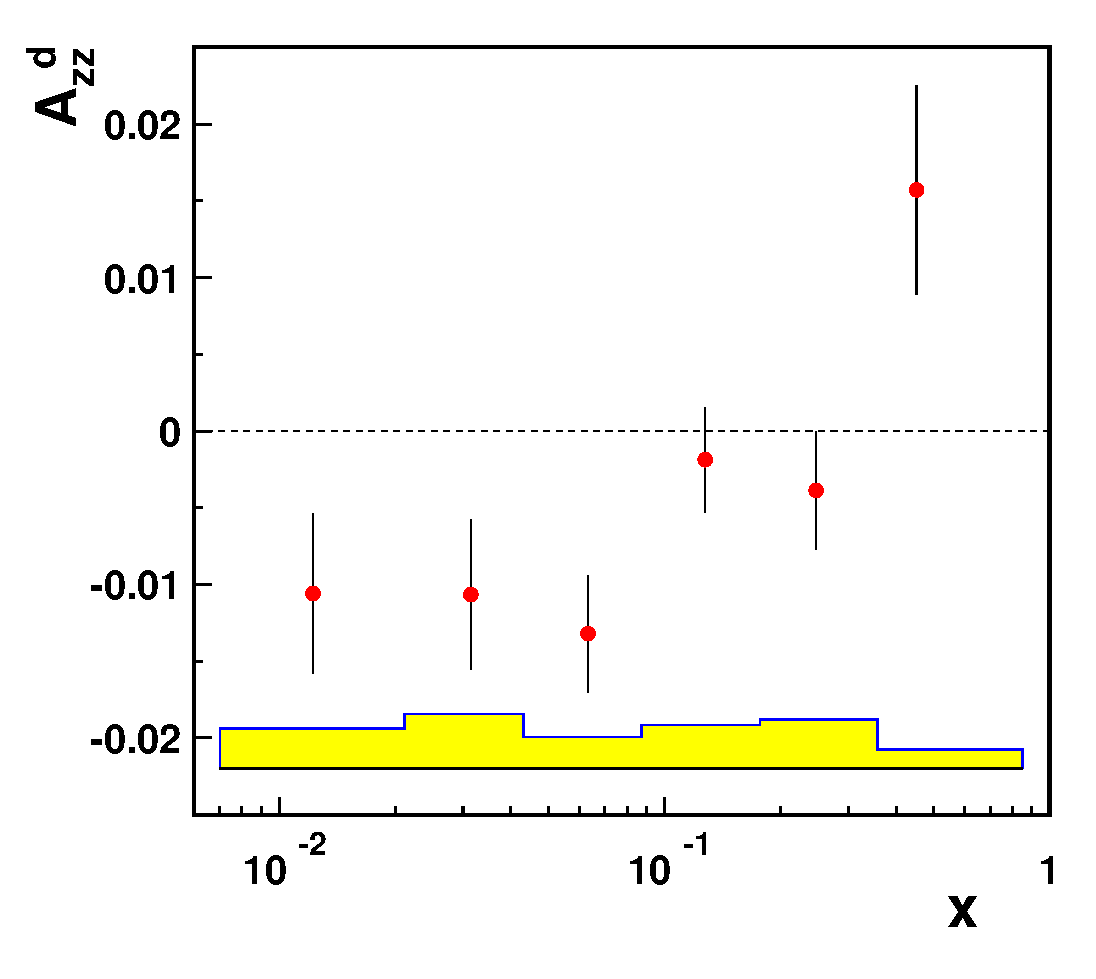
\includegraphics[angle=0,width=4.in]{figs/azzfinal.eps}
%\caption{\label{HERMES_AZZ} HERMES measurement of the inclusive tensor asymmetry A$_{zz}$ of the deuteron.
%The error band displays the total systematic uncertainty.
%{\it Reproduced from~\cite{Riedl:2005jq}.}}
%\end{center}\end{figure}

%\begin{figure}
%\begin{center}
%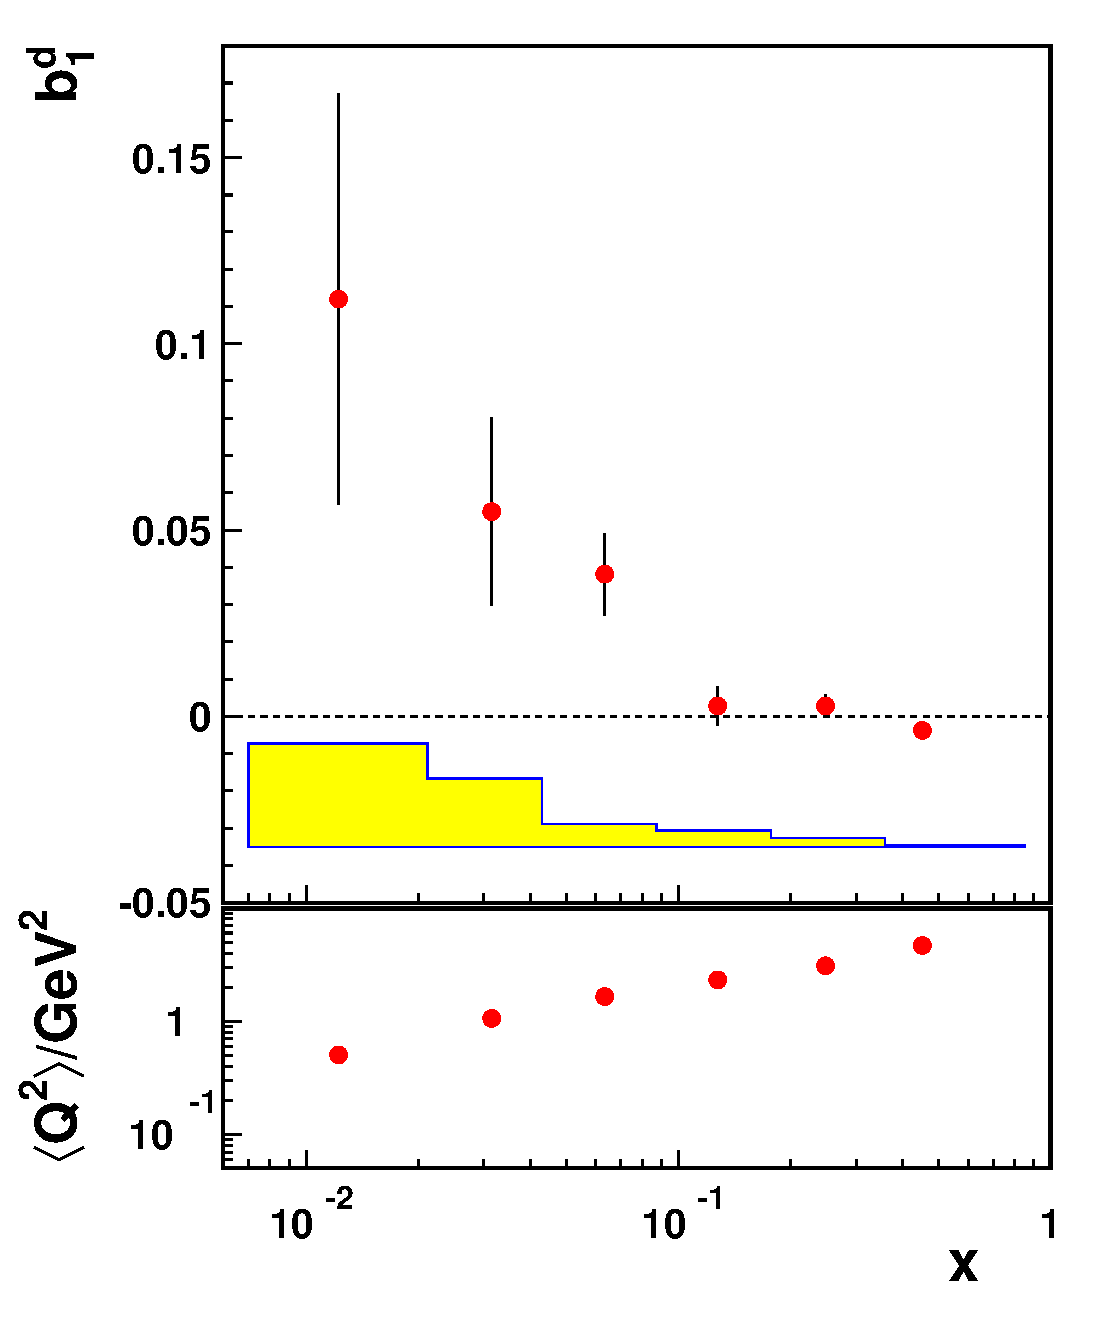
\includegraphics[angle=0,width=4.1in]{figs/b1final.eps}
%\caption{\label{HERMES_B1D} HERMES measurement of the inclusive tensor structure function b$_1^d$ and the average $Q^2$ for each x-bin.  The error band displays the total systematic uncertainty.
%{\it Reproduced from~\cite{Riedl:2005jq}.}}
%\end{center}\end{figure}


\begin{figure}
\begin{center}
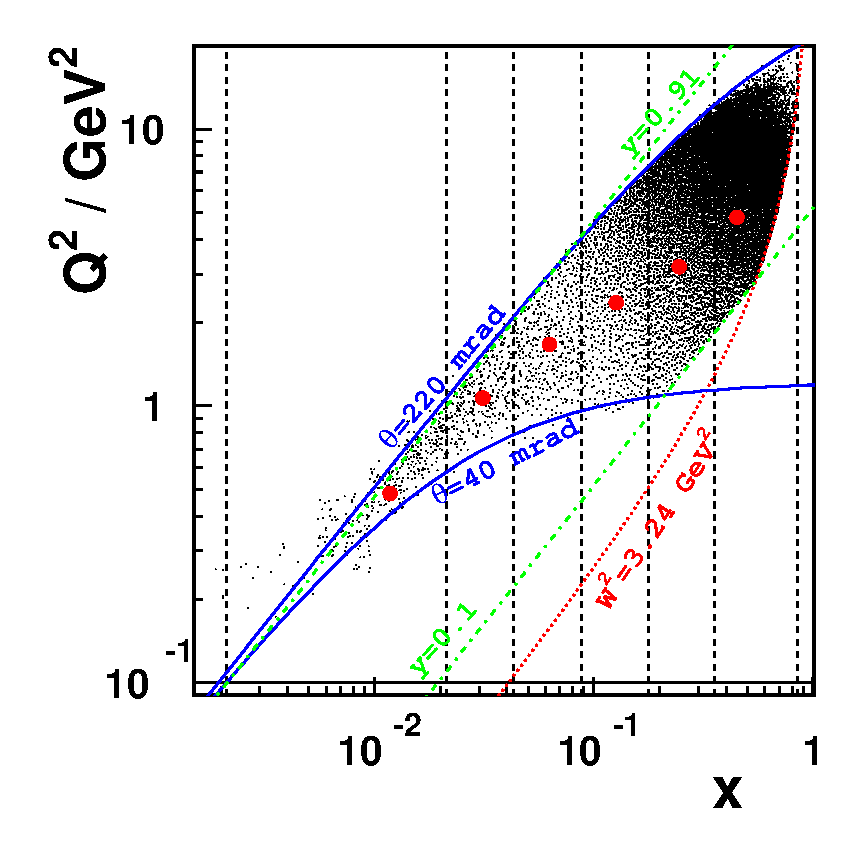
\includegraphics[angle=0,width=0.45\textwidth]{figs/kineplane.eps}
\caption{\label{HERMES_KIN} Kinematic coverage of the HERMES measurement.  The dashed vertical lines indicate the borders
of the bins in x, the dots their centers of gravity. The solid curves
indicate the
vertical acceptance of the spectrometer, defined by its aperture.
In addition, the
kinematic cuts imposed on the variables Q$^2$, y
and W$^2$ are shown. 
%The W$^2$ cut suppresses the nuclear resonance region.
{\it Reproduced from~\cite{Riedl:2005jq}.}}
\end{center}\end{figure}


The HERMES collaboration  made the first measurement~\cite{Riedl:2005jq,Airapetian:2005cb} of
$b_1$ in 2005.
The experiment explored the low $x$ region of $0.001<x<0.45$ for  $0.5<Q^2<5$ GeV$^2$.  
An atomic beam source was used to generate a deuterium gas target with high tensor polarization.  
The HERA storage ring provided 27.6 GeV positrons incident on the internal gas target.

As displayed in Fig.~\ref{HERMES_AZZ}, the tensor asymmetry A$_{zz}$  was found to be 
non-zero at about the  two sigma level, with an apparent zero crossing around $x=0.3$. %  for $x < 0.1$.  
%
The tensor structure function $b_1$ exhibits a steep rise as $x\to 0$, which is qualitatively
in agreement with the predictions of coherent double-scattering models. See for example Ref.~\cite{Edelmann:1997ik}.  The authors of Ref.~\cite{Airapetian:2005cb} interpret the rapid rise at low $x$ in terms of the same mechanism that leads to nuclear shadowing in unpolarized scattering, i.e. double scattering of the lepton, first from the proton, then from the neutron, with sensitivity to the spatial alignment of the two nucleons.
%The Close-Kumano integral (Eq.~\ref{cksum}) was evaluated and found to be:
%\begin{eqnarray}
%\int_{0.0002}^{0.85} b_1(x) dx = 0.0105 \pm 0.0034 \pm 0.0035
%\end{eqnarray}
%which result possibly indicates a breaking of the Close-Kumano sum rule, and consequently a 
%tensor-polarized quark sea.
%%
%%

As is often the case with a pioneer measurement, the precision of the results leaves some
room for ambiguity.  Despite the surprisingly large magnitude and interesting trend of the data, 
all points are roughly within two sigma from zero, which calls for a higher precision measurement.
Another issue is that some of the HERMES momentum transfer values are low 
(see Fig.~\ref{HERMES_KIN}), so that quark structure functions may not be the correct language. 
The $Q^2$ variation in each $x$-bin is also quite wide ($\approx$10 GeV$^2$ for $x\sim 0.3$), which complicates
the interpretation of this data, since  several models predict significant $Q^2$-dependence of
 $b_1$. See for example Fig.~\ref{xb1_pred}.


%\begin{figure}\begin{center}
%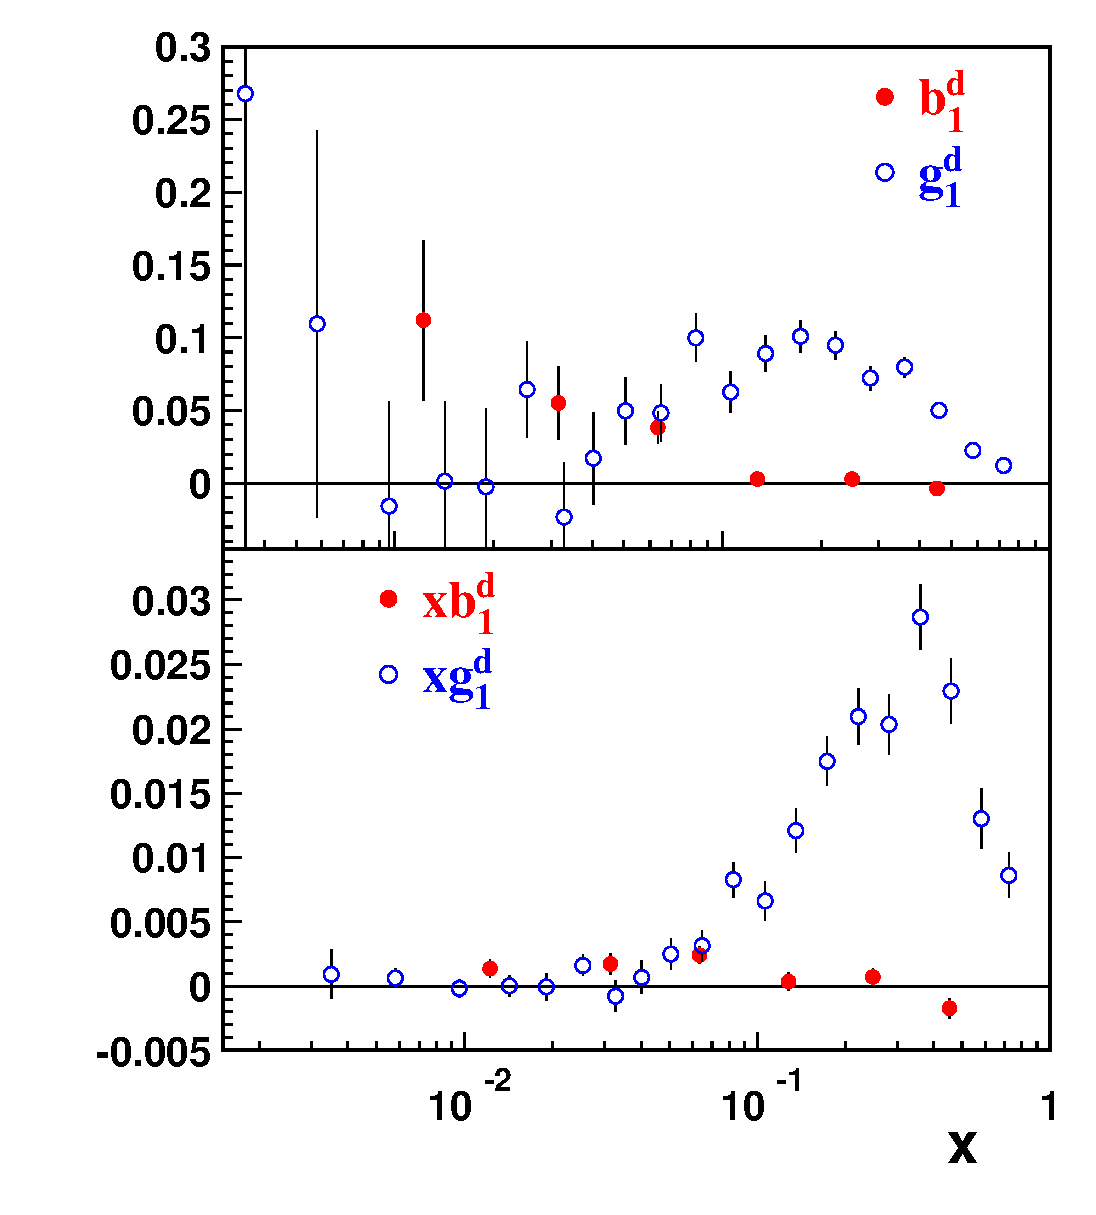
\includegraphics[angle=0,width=3.1in]{figs/b1g1.eps}
%\caption{\label{}\footnotesize
%{\it Reproduced from~\cite{Riedl:2005jq}.}}
%\end{center}\end{figure}

%\begin{figure}\begin{center}
%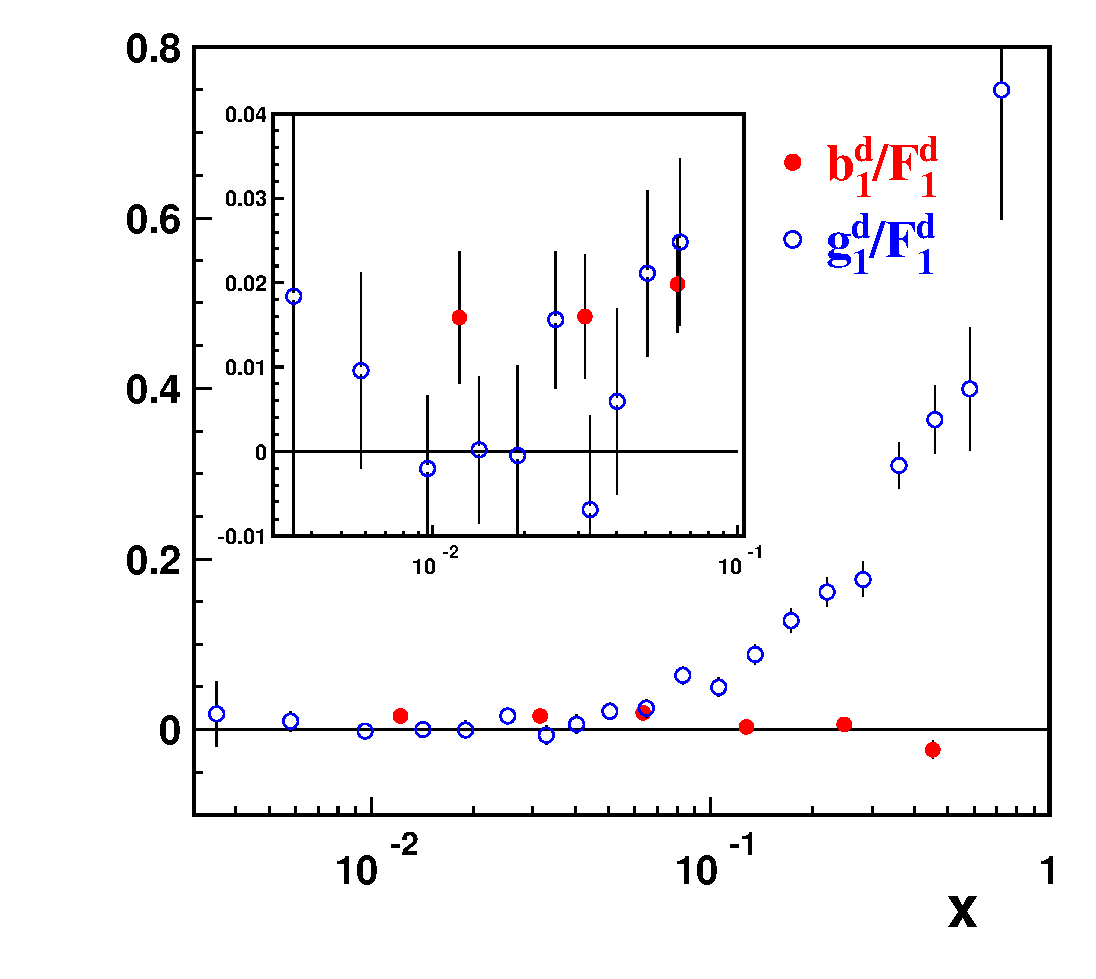
\includegraphics[angle=0,width=3.1in]{figs/b1g1overf1.eps}
%caption{\label{}\footnotesize
%{\it Reproduced from~\cite{Riedl:2005jq}.}}
%\end{center}\end{figure}

%\begin{figure}\begin{center}
%\includegraphics[angle=0,width=3.1in]{figs/b2theo.eps}
%\caption{\label{}\footnotesize
%{\it Reproduced from~\cite{Riedl:2005jq}.}}
%\end{center}\end{figure}


%%%%%%%%%%%%%
%%%%%%%%%%%%%
\subsubsection{Interpretation in the Operator Product Expansion}
%
In the Operator Product Expansion (OPE) framework, the leading operators 
$O_V^{\mu_1...\mu_n}$ and $O_A^{\mu_1...\mu_n}$ in the expansion are twist two. For a 
spin-1 target, the matrix elements of the time-ordered product of two currents 
$T_{\mu\nu}$ have the following expressions:
%
\begin{eqnarray}
<p,E|O_V^{\mu_1...\mu_n}|p,E>&=&S[a_np^{\mu_1}...p^{\mu_n}+d_n(E^{*\mu_1}E^{\mu_2}-\frac{1}{3}p^{\mu_1}
p^{\mu_2})p^{\mu_3}...p^{\mu_n}], \nonumber \\
<p,E|O_A^{\mu_1...\mu_n}|p,E>&=&S[r_n\epsilon^{\lambda\sigma\tau\mu_1}E_{\lambda}^*E_{\sigma}p_{\tau}
p^{\mu_2}...p^{\mu_n}]
\label{matrix-elt}
\end{eqnarray}
%
The non-zero value of $b_1$ arises from the fact that, in a spin-1 target, the 
$\frac{1}{3}p^{\mu_1}p^{\mu_2}$ term doesn't cancel the tensor structure $E^{*\mu_1}E^{\mu_2}$. 
The coefficient $d_n$ can be extracted from the comparison of $T_{\mu\nu}$ expansion 
and the spin-1 target hadronic tensor Eq.~\ref{had-tensor} as follows:
%
\begin{eqnarray}
b_1(\omega)&=&\sum_{n=2,4,...}^\infty 2 C_n^{(1)} d_n \omega^n, \nonumber \\
b_2(\omega)&=&\sum_{n=2,4,...}^\infty 4 C_n^{(2)} d_n \omega^{n-1},
\end{eqnarray}
%
for $1 \le |\omega| \le \infty$ (where $\omega = 1/x$). A Callan-Gross-type relation 
exists for the two leading order tensor structure functions:
%
\begin{eqnarray}
 2 x b_1 = b_2
\label{callan-gross}
\end{eqnarray}
%
valid at lowest order of QCD, where $C_n^{(1)} = C_n^{(2)}$.
At higher orders, Eq.~\ref{callan-gross} is violated.

Sum rules can be 
extracted from the moments of the tensor structure functions:
%
\begin{eqnarray}
\int_0^1 x^{n-1}~b_1(x)~dx &=& \frac{1}{2}~C_n^{(1)}~d_n, \nonumber \\
\int_0^1 x^{n-2}~b_2(x)~dx &=& C_n^{(2)}~d_n,
\label{sr}
\end{eqnarray}
%
where n is even. 

The OPE formalism is based on QCD and is target-independent. However, a target dependence 
is generated by Eq.~\ref{matrix-elt}, and spin-1 structure functions are subject to 
the same QCD corrections and their moments have the same anomalous dimensions as for 
a spin-1/2 target. In addition, the tensor structure functions should exhibit the same 
scaling behavior as $F_1$ and $F_2$, since they are generated from the same matrix 
element $O_V^{\mu_1...\mu_n}$.

We focus in this document on the leading twist structure function $b_1$.  A Callan-Gross type relation allows access to $b_2$ once $b_1$ is determined, and $b_3$ and $b_4$ do not contribute at leading twist.
%%%%%%%%
%%%%%%%%
\subsubsection{Interpretation in the Parton Model}
%
In the infinite momentum frame\footnote{All spins and
momenta are along the $z$-axis.} of the parton model, 
the scattering of the virtual photon from a free quark 
with spin up (or down), which carries a momentum fraction $x$ of the spin-$m$ hadron, can be 
expressed through the hadronic tensor $W_{\mu\nu}^{(m)}$:
%
\begin{eqnarray}
W_{\mu\nu}^{(1)} = \Bigg(- \frac{1}{2} g_{\mu\nu} + \frac{x}{\nu} P_{\mu}P{\nu}\Bigg) 
                               \Big(q^1_{\uparrow}(x) + q^1_{\downarrow}(x)\Big) \nonumber
                    + \frac{i \epsilon_{\mu\nu\lambda\sigma} q^{\lambda} s^{\sigma}}{2 \nu} 
                               \Big(q^1_{\uparrow}(x) - q^1_{\downarrow}(x)\Big),
\label{had-tensor-1}
\end{eqnarray}
%
for a target of spin projection equal to 1 along the $z$-direction, and:
%
\begin{eqnarray}
W_{\mu\nu}^{(0)} = \Bigg(- \frac{1}{2} g_{\mu\nu} + \frac{x}{\nu} P_{\mu}P{\nu}\Bigg) 
                               2 q^0_{\uparrow}(x) 
\label{had-tensor-0}
\end{eqnarray}
%
for a target of spin projection equal to zero along the $z$-direction. The tensor 
structure functions $b_1$ and $b_2$ can be expressed from the comparison of 
$W_{\mu\nu}^{(1)} - W_{\mu\nu}^{(0)}$ with Eq.~\ref{had-tensor} as follows:
%
\begin{eqnarray}
b_1(x) &=& \frac{1}{2} \Big( 2 q^0_{\uparrow}(x) - q^1_{\uparrow}(x) - q^1_{\downarrow}(x) \Big) \\
b_2(x) &=& 2 x b_1(x)
\label{TSF-parton}
\end{eqnarray}
%
where $q^m_{\uparrow}$ ($q^m_{\downarrow}$)  represents the probability to find a quark with momentum fraction $x$ and spin up (down) in a hadron which is in helicity state $m$.
%For example, $q^1_{\uparrow}(x)$ is the probability to find a quark with spin up and momentum fraction $x$ in a deuteron that is in state $m=1$. 
%
The tensor structure function $b_1$ depends only on the spin-averaged parton distributions\footnote{since, by parity, $q^m_{\uparrow}= q^m_{\downarrow}$} 
\begin{eqnarray*}
q^1(x) &=& q^1_{\uparrow}(x) + q^1_{\downarrow}(x)\\ 
q^0(x) &=& q^0_{\uparrow}(x) + q^0_{\downarrow}(x) 
= 2 q^0_{\uparrow}(x)
\end{eqnarray*}
so it can be expressed as:
\begin{eqnarray}
b_1(x) = \frac{q^0(x) - q^1(x)}{2}
\end{eqnarray}

Explicitly, $b_1$ measures the difference
in partonic constituency in an $|m|$=1 target and an $m$=0 target. 
 From this we see that while $b_1$ is defined in terms of quark distributions, it interestingly depends also on the spin state of the nucleus as a whole.

%The three leading twist structure functions are $F_1$, $g_1$ and $b_1$.
%The tensor structure function $b_1$, which is leading-twist like  $F_1$ and 
%$g_1$, is quite interesting, in that it presents a simple gauge of nuclear 
%effects: $b_1$ would vanish if the deuteron was simply a proton and neutron in 
%a relative S state.
%
%
%%The Hermes collaboration  made a first measurement~\cite{Airapetian:2005cb} of 
%$b_1$ and found significantly non-zero results.  Beyond providing insight into
%nuclear structure, this has the potential to impact $g_1^n$ and $g_2^n$ extractions, 
%where $b_1$ has traditionally been ignored when the neutron is extracted from 
%deuteron data.






\subsubsection{First Measurement of $b_1(x)$ by the HERMES Collaboration}
 \label{B1DATASECTION}
%\begin{figure}
%\begin{center}
%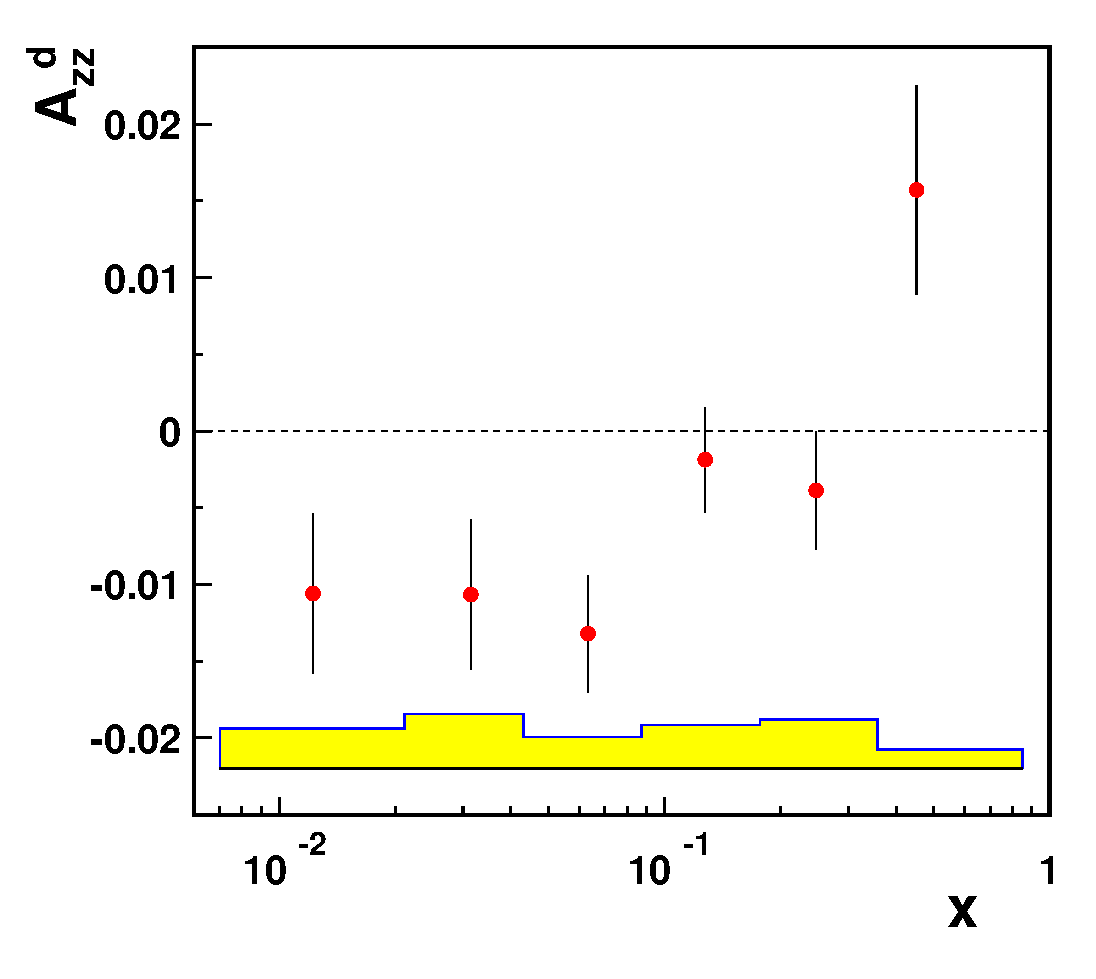
\includegraphics[angle=0,width=0.45\textwidth]{figs/azzfinal.eps}
%
%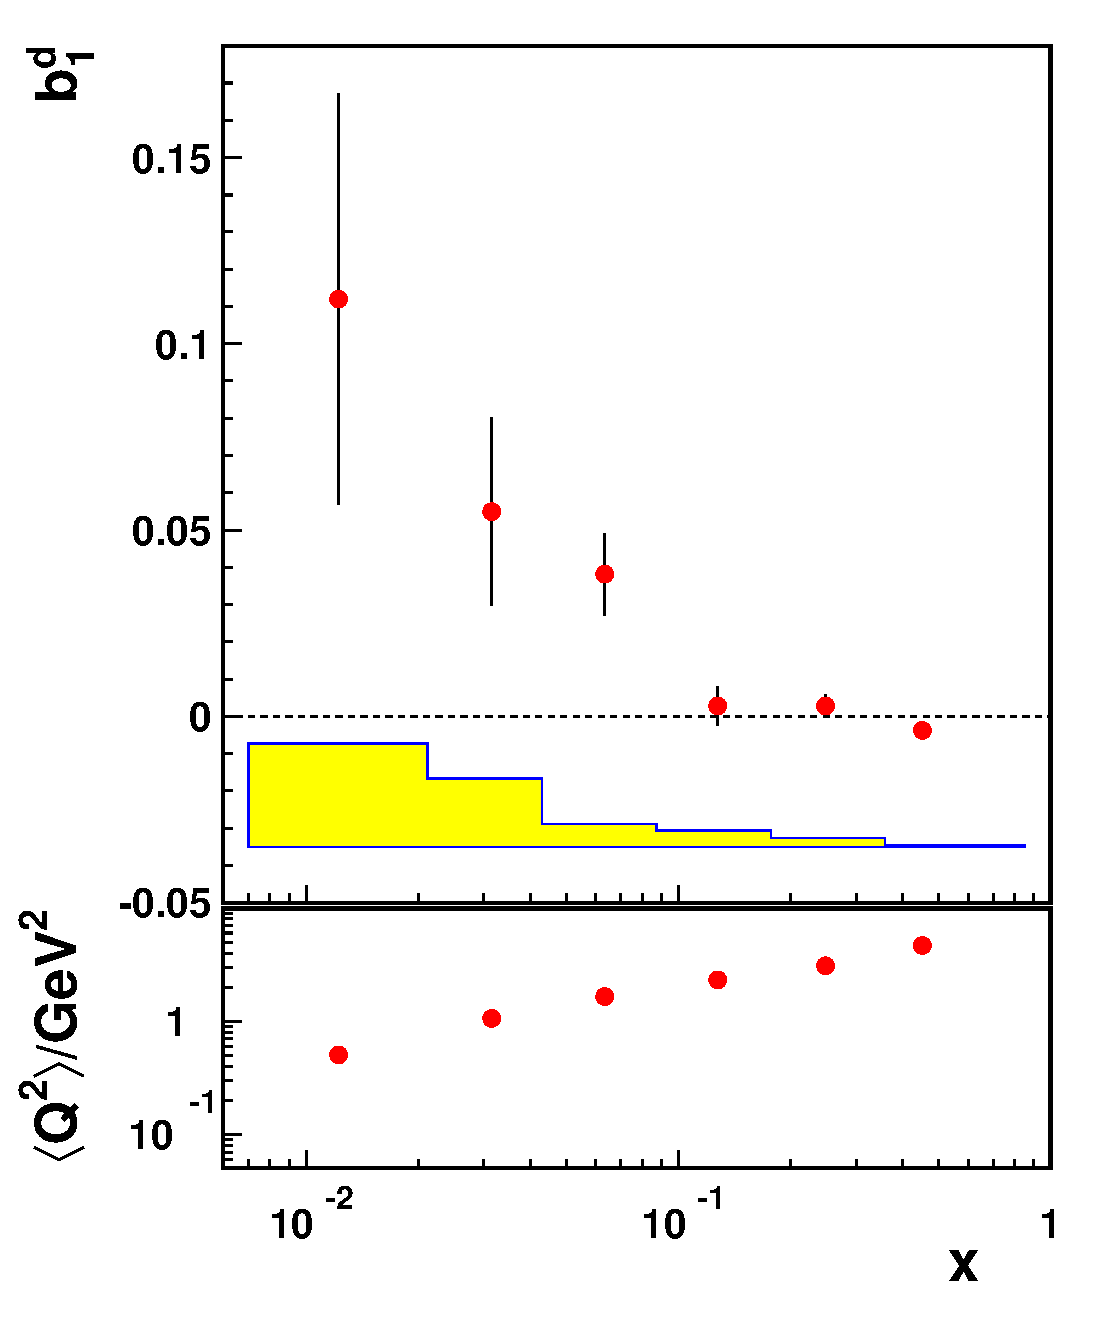
\includegraphics[angle=0,width=0.47\textwidth]{figs/b1final.eps}
%\caption{\label{HERMES_AZZ} {\bf Top:} HERMES measurement of the inclusive tensor asymmetry A$_{zz}$ of the deuteron.  
%{\bf Bottom:} HERMES measurement of the inclusive tensor structure function b$_1^d$ and the average $Q^2$ for each x-bin.  The error bands displays the total systematic uncertainty.
%{\it Reproduced from~\cite{Riedl:2005jq}.}}
%\end{center}\end{figure}

\begin{figure}
\begin{center}
\includegraphics[angle=0,width=0.45\textwidth]{figs/1.eps}
\hspace{0.5cm}
\includegraphics[angle=0,width=0.45\textwidth]{figs/2.eps}
\vspace{3cm}

\includegraphics[angle=0,width=0.45\textwidth]{figs/3.eps}
\caption{\label{HERMES_AZZ} {\bf Top}: HERMES~\cite{Riedl:2005jq} measurement of the inclusive tensor asymmetry A$_{zz}(x)$ and $xb_1(x)$ of the deuteron. {\bf Bottom} : The tensor structure function $b_1(x)$ without $x$-weighting, which reveals a steep rise as $x\to 0$. 
}
\end{center}\end{figure}

%\begin{figure}
%\begin{center}
%\includegraphics[angle=0,width=0.47\textwidth]{figs/2.eps}
%\caption{\label{HERMES_AZZ2} 
%HERMES~\cite{Riedl:2005jq} measurement of the inclusive tensor structure function b$_1^d$.  
%}
%\end{center}\end{figure}



%\begin{figure}
%\begin{center}
%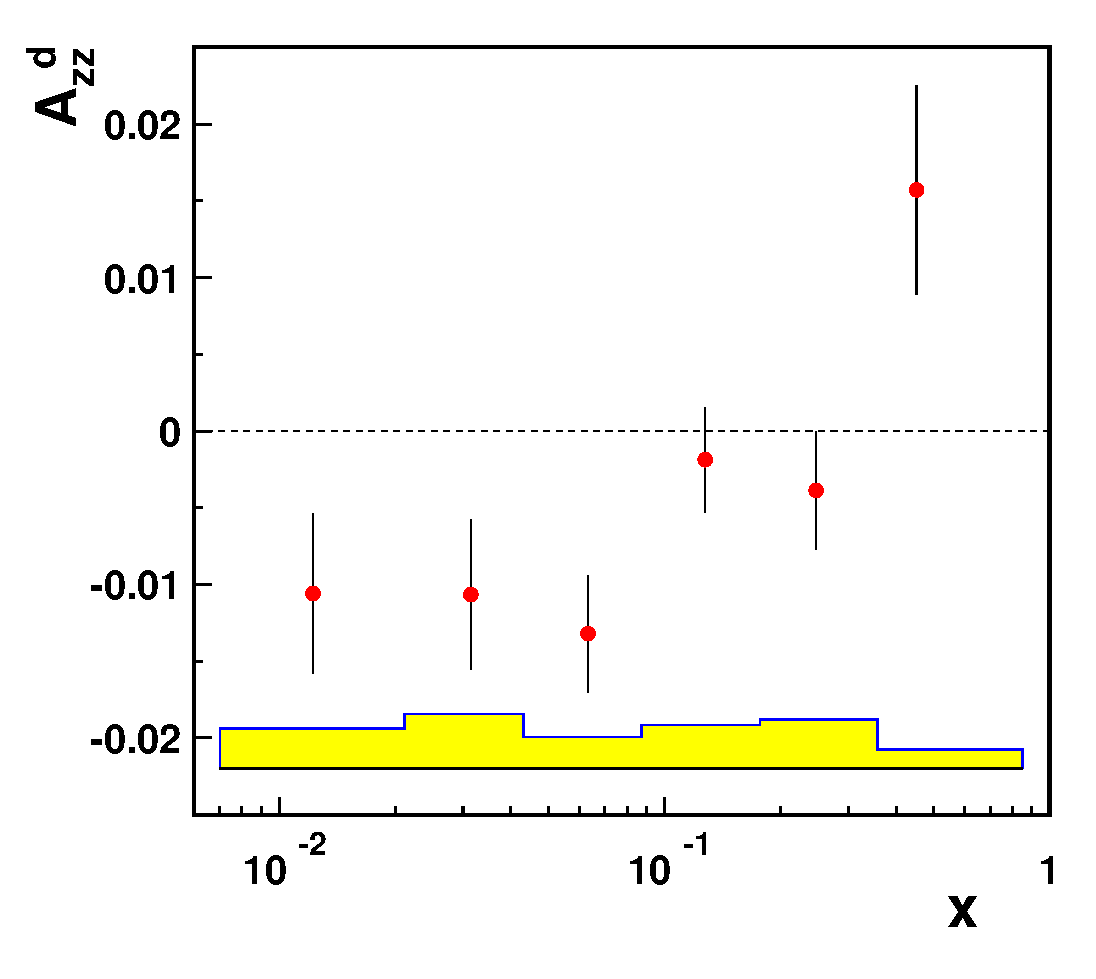
\includegraphics[angle=0,width=4.in]{figs/azzfinal.eps}
%\caption{\label{HERMES_AZZ} HERMES measurement of the inclusive tensor asymmetry A$_{zz}$ of the deuteron.
%The error band displays the total systematic uncertainty.
%{\it Reproduced from~\cite{Riedl:2005jq}.}}
%\end{center}\end{figure}

%\begin{figure}
%\begin{center}
%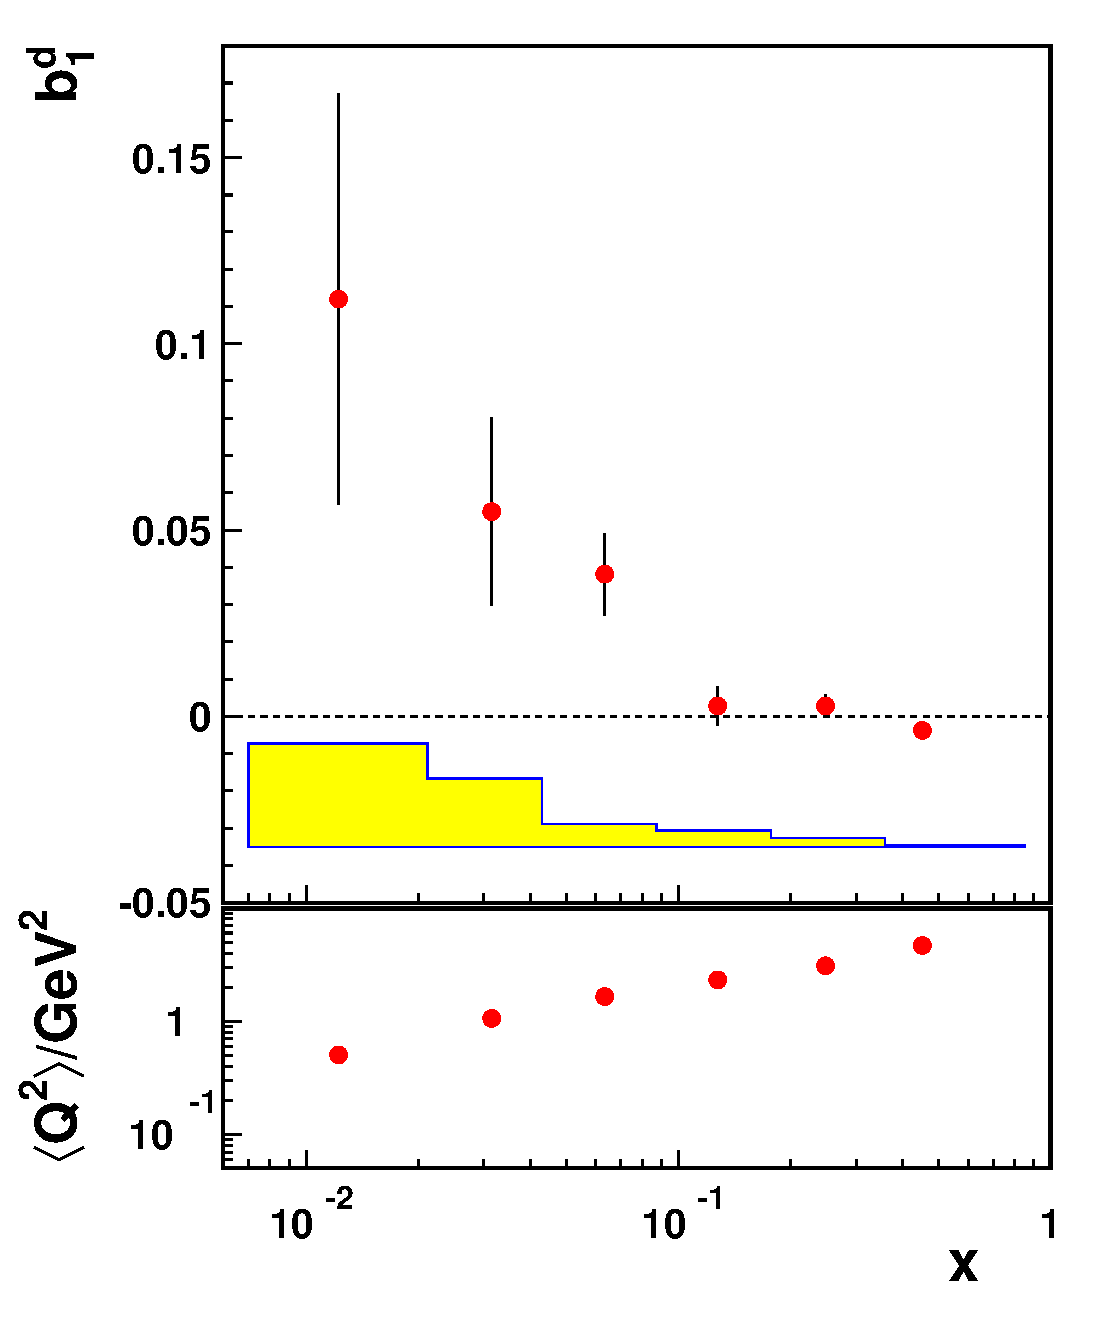
\includegraphics[angle=0,width=4.1in]{figs/b1final.eps}
%\caption{\label{HERMES_B1D} HERMES measurement of the inclusive tensor structure function b$_1^d$ and the average $Q^2$ for each x-bin.  The error band displays the total systematic uncertainty.
%{\it Reproduced from~\cite{Riedl:2005jq}.}}
%\end{center}\end{figure}


\begin{figure}
\begin{center}
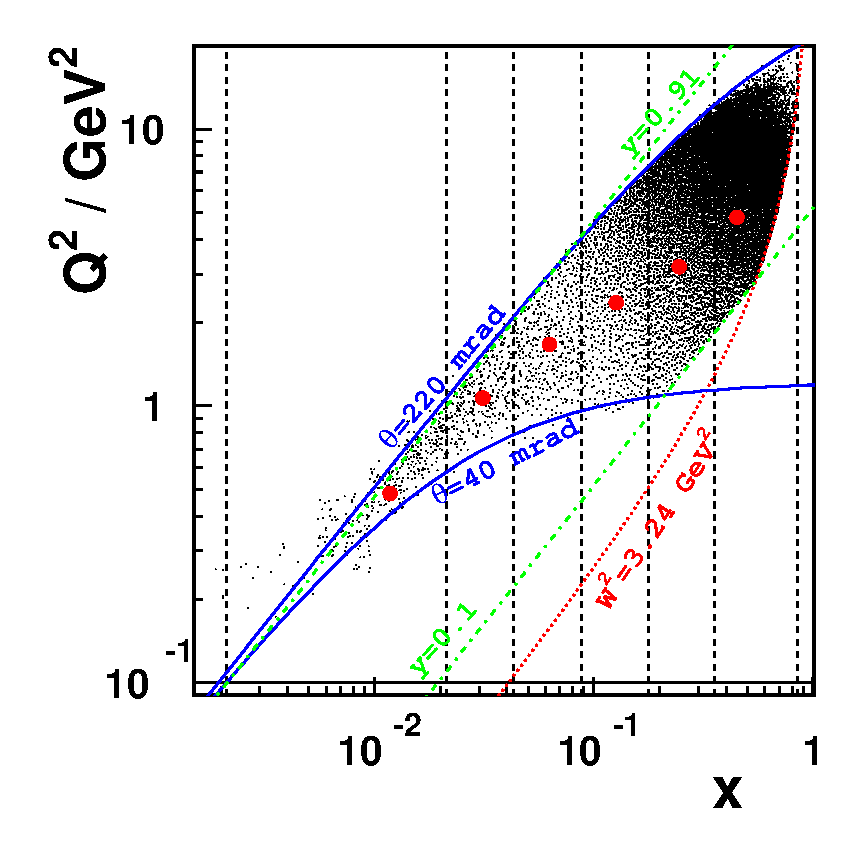
\includegraphics[angle=0,width=0.45\textwidth]{figs/kineplane.eps}
\caption{\label{HERMES_KIN} Kinematic coverage of the HERMES measurement.  The dashed vertical lines indicate the borders
of the bins in x, the dots their centers of gravity. The solid curves
indicate the
vertical acceptance of the spectrometer, defined by its aperture.
In addition, the
kinematic cuts imposed on the variables Q$^2$, y
and W$^2$ are shown. 
%The W$^2$ cut suppresses the nuclear resonance region.
{\it Reproduced from~\cite{Riedl:2005jq}.}}
\end{center}\end{figure}


The HERMES collaboration  made the first measurement~\cite{Riedl:2005jq,Airapetian:2005cb} of
$b_1$ in 2005.
The experiment explored the low $x$ region of $0.001<x<0.45$ for  $0.5<Q^2<5$ GeV$^2$.  
An atomic beam source was used to generate a deuterium gas target with high tensor polarization.  
The HERA storage ring provided 27.6 GeV positrons incident on the internal gas target.

As displayed in Fig.~\ref{HERMES_AZZ}, the tensor asymmetry A$_{zz}$  was found to be 
non-zero at about the  two sigma level, with an apparent zero crossing around $x=0.3$. %  for $x < 0.1$.  
%
The tensor structure function $b_1$ exhibits a steep rise as $x\to 0$, which is qualitatively
in agreement with the predictions of coherent double-scattering models. See for example Ref.~\cite{Edelmann:1997ik}.  The authors of Ref.~\cite{Airapetian:2005cb} interpret the rapid rise at low $x$ in terms of the same mechanism that leads to nuclear shadowing in unpolarized scattering, i.e. double scattering of the lepton, first from the proton, then from the neutron, with sensitivity to the spatial alignment of the two nucleons.
%The Close-Kumano integral (Eq.~\ref{cksum}) was evaluated and found to be:
%\begin{eqnarray}
%\int_{0.0002}^{0.85} b_1(x) dx = 0.0105 \pm 0.0034 \pm 0.0035
%\end{eqnarray}
%which result possibly indicates a breaking of the Close-Kumano sum rule, and consequently a 
%tensor-polarized quark sea.
%%
%%

As is often the case with a pioneer measurement, the precision of the results leaves some
room for ambiguity.  Despite the surprisingly large magnitude and interesting trend of the data, 
all points are roughly within two sigma from zero, which calls for a higher precision measurement.
Another issue is that some of the HERMES momentum transfer values are low 
(see Fig.~\ref{HERMES_KIN}), so that quark structure functions may not be the correct language. 
The $Q^2$ variation in each $x$-bin is also quite wide ($\approx$10 GeV$^2$ for $x\sim 0.3$), which complicates
the interpretation of this data, since  several models predict significant $Q^2$-dependence of
 $b_1$. See for example Fig.~\ref{xb1_pred}.


%\begin{figure}\begin{center}
%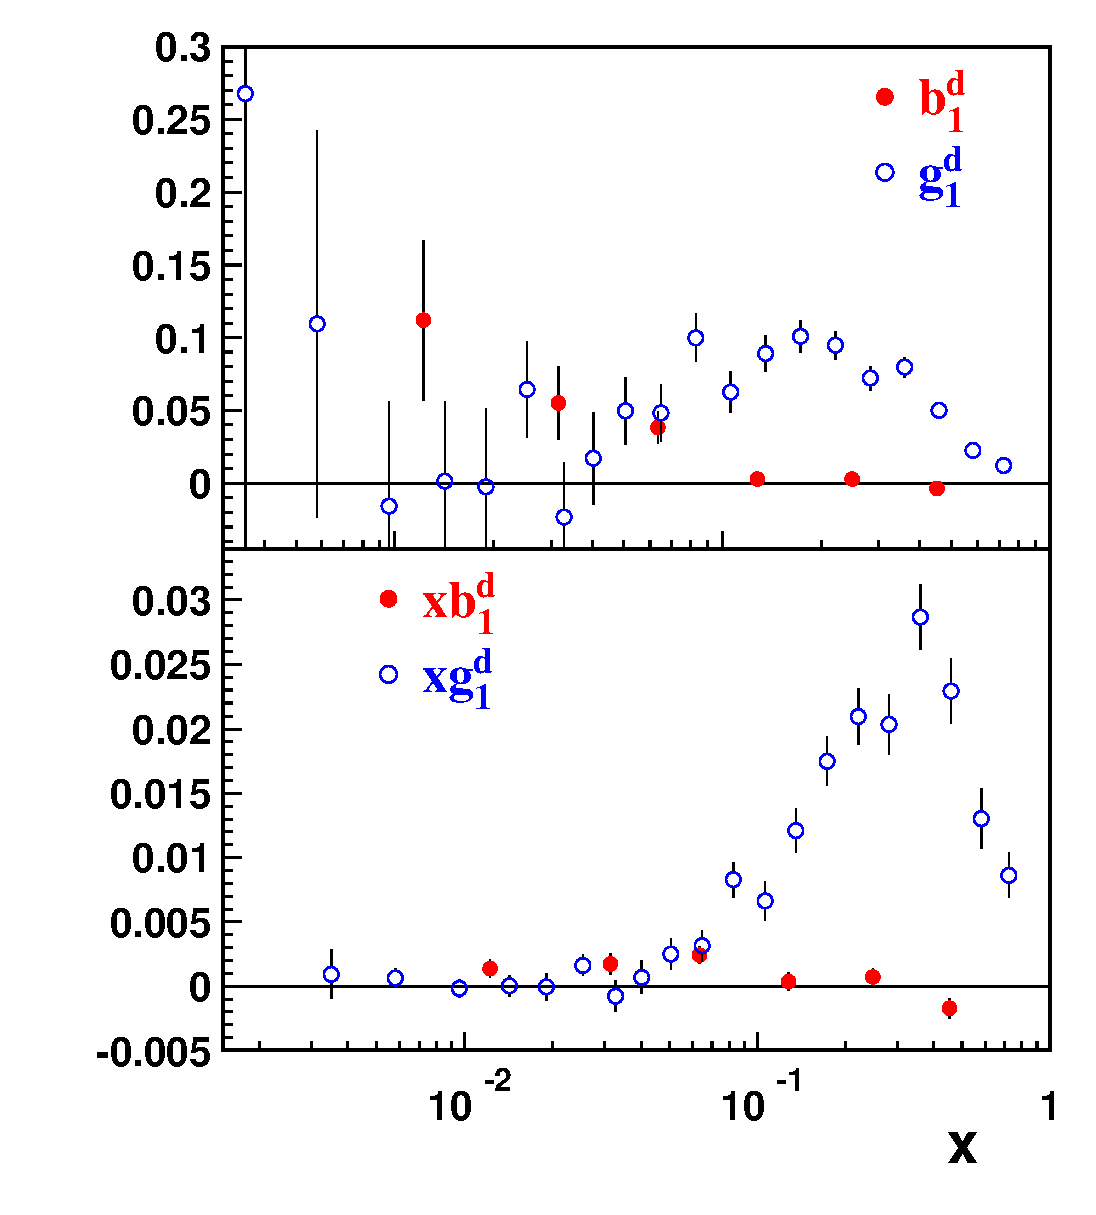
\includegraphics[angle=0,width=3.1in]{figs/b1g1.eps}
%\caption{\label{}\footnotesize
%{\it Reproduced from~\cite{Riedl:2005jq}.}}
%\end{center}\end{figure}

%\begin{figure}\begin{center}
%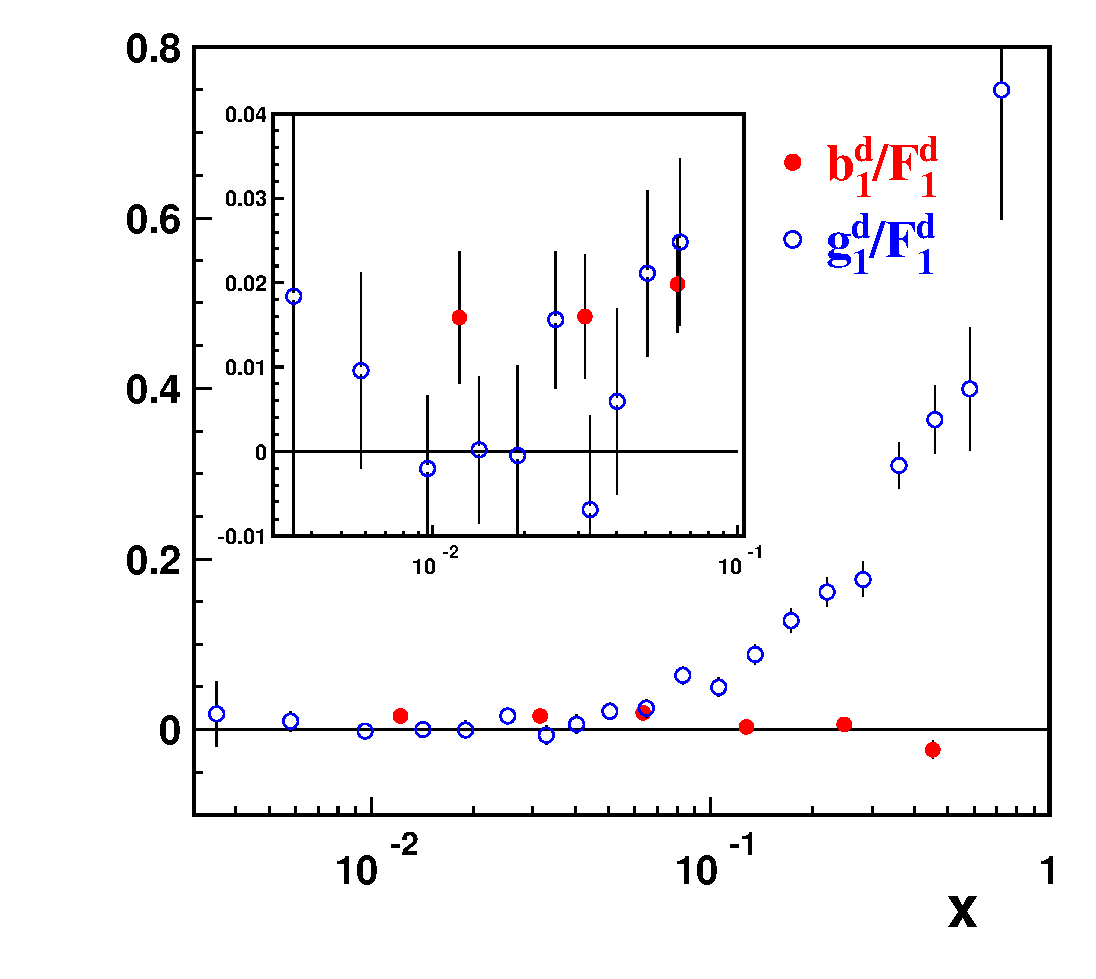
\includegraphics[angle=0,width=3.1in]{figs/b1g1overf1.eps}
%caption{\label{}\footnotesize
%{\it Reproduced from~\cite{Riedl:2005jq}.}}
%\end{center}\end{figure}

%\begin{figure}\begin{center}
%\includegraphics[angle=0,width=3.1in]{figs/b2theo.eps}
%\caption{\label{}\footnotesize
%{\it Reproduced from~\cite{Riedl:2005jq}.}}
%\end{center}\end{figure}



\subsection{Predictions for the Tensor Structure Function $b_1(x)$}
\label{PREDB1X}
   %%
The leading twist tensor structure function $b_1$ quantifies effects not present in 
the case of spin-half hadrons. However the only available targets to study the 
tensor polarization effects on the nucleon substructure are nuclei. 
A measurement of $b_1$ would allow us to take 
a deeper look at the nucleus internal dynamics as $b_1$ should be zero if the 
nucleus is made up of spin-half constistuents at rest, or in a relative $s$-wave. 
Therefore a non-negligible value of $b_1$ can be understood in terms of the deviation 
of a nucleus from a simple bound state of protons and neutrons.
%
\subsubsection{Conventional Nuclear Effects}
The deuteron is the simplest spin-1 many-body nuclear system. In Ref.~\cite{Hoodbhoy:1988am},
the authors evaluate the value of $b_1$ in three different scenarios for the deuteron
constituents and their dynamics:
\begin{enumerate}
 \item[I.] The deuteron is composed of two spin-1/2 non-interacting nucleons at rest. 
In this case, the eight helicity amplitudes characteristic of a spin-1 target are 
expressed in terms of the four helicity amplitudes of each spin-1/2 nucleons, and 
therefore the total number of independent amplitudes is reduced from eight to four. All structure 
functions of the deuteron are then the simple sum of the structure functions of the two 
nucleons, and the tensor structure functions vanish: $b_1 = b_2 
= b_3 = b_4 = 0$. 
 \item[II.] The deuteron is composed of two spin-1/2 nucleons moving non-relativistically 
in a central potential. The target motion modifies the helicity amplitudes. Using
the convolution formalism, it was found that the contribution of these moving nucleons
to $b_1$ is small and is dominated by the lower component of the nucleon's Dirac
wave function.
 \item[III.] The deuteron contains a $D$-state admixture. Because the proton and the neutron
are moving in opposite directions, an additional term due to the $S-D$ interference 
appears in the convolution procedure. This extra contribution to $b_1$ is predicted
to be even smaller than in the previous case.
\end{enumerate}

However, at the quark level, when considering the case of massless relativistic quark, 
$b_1$ exhibits very large negative values peaked at $x=0.5$~\cite{Hoodbhoy:1988am}.
In this calculation, a meson in the $j=1$ state is formed from the coupling of a $P_{3/2}$ 
massless quark with a spin-1/2 spectator.

\begin{figure}[t]
\begin{center}
%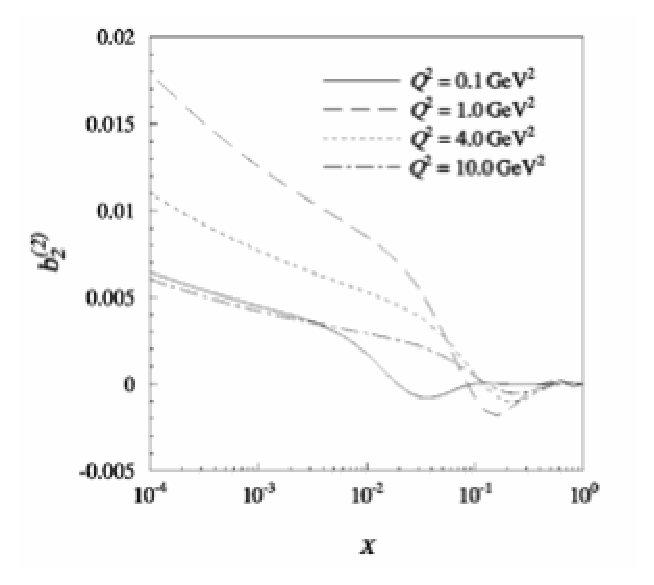
\includegraphics[width=0.40\textwidth]{figs/bora_jaffe_fig3.eps}
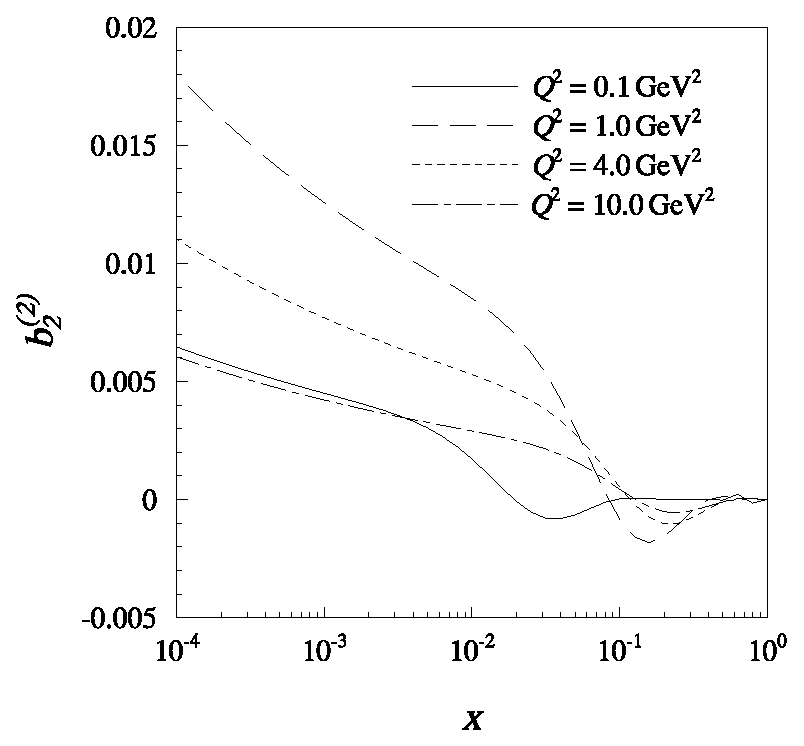
\includegraphics[width=0.3725\textwidth]{figs/bx.eps}
\hspace{0.3cm}
\includegraphics[width=0.45\textwidth]{figs/xb1_mstw_newmiller.eps}
\caption{\label{xb1_pred} Theoretical predictions. {\bf Left plot:} Double-scattering 
contribution to $b_2(x,Q^2)$ as a  function of $x$~\cite{Bora:1997pi}.  Note the strong $Q^2$ dependence at low x.
%($b_2 = b_2^{(1)}+b_2^{(2)}$). 
{\bf Right plot:} HERMES results~\cite{Airapetian:2005cb} compared to calculations 
from S.~Kumano~\cite{Kumano:2010vz} and from the one-pion exchange effects of 
G. Miller~\cite{Miller:1989nc,Miller_tmp}.}
\end{center}
\end{figure}

In 1988, Miller also examined the tensor structure function $b_1$~\cite{Miller:1989nc}.
The basic mechanism is that the virtual photon hits an exchanged pion  which
is responsible for the binding of the deuteron. The calculation depends on the pion 
structure function which carries uncertainty. 
In this early calculation, the convention used by Miller was different from the
one used in the HERMES results and in Ref.~\cite{Kumano:2010vz}. The updated 
calculation~\cite{Miller_tmp} is shown in Fig.~\ref{xb1_pred}. Also the pion structure 
function from~\cite{Sutton:1991ay} was used. The spread of the curve originates from the 
parameter $A_s=(.9 \pm 0.3)$ which governs the strength of the sea in the pion. These 
numbers are all in qualitative agreement with HERMES, given their large error bars.
Another mechanism is expecting to contribute: coherent-double scattering. Miller 
specified that his mechanism is not the same as that, even though the HERMES 
publication~\cite{Airapetian:2005cb} combined them together.

In addition, at $x > 0.2$, a non-negligible value of $b_1^d$ is expected just through
the conventional nuclear effects in the deuteron, Fermi motion and binding~\cite{Khan:1991qk}.

%
\subsubsection{Double-Scattering Effects}
%This leading twist structure function quantifies effects not present
%in the case of spin-half hadrons. It allows a deeper look at the nucleus internal 
%dynamics as $b_1$ should be zero if the nucleus is made up of spin-half constistuents 
%at rest, or in a relative $s$-wave. Therefore a non-negligible value of $b_1$ can be 
%translated into the deviation of a nucleus from a simple bound state of protons and 
%neutrons.
%
Using Vector Meson Dominance (VMD), the authors of Ref.~\cite{Bora:1997pi} isolate the 
double-scattering contribution to $b_1$. The existence time of a vector meson can 
be described by the coherence length $\lambda$: 
\begin{eqnarray}
\lambda = \frac{Q^2}{M x (M_v^2 + Q^2)}
\end{eqnarray}
which is the length over which the vector meson propagates during the time $\Delta t 
= 1/\Delta E$. Therefore, for multiple scattering to occur, a minimum coherence length 
of $\approx$ 1.7 fm (the inter-nucleon separation) is required. At 
$x > 0.3$, the coherence length is only about the size of the nucleon, so multiple 
scattering contributions are anticipated to be negligible. However, for $x \le 0.1$, 
double-scattering should be significant in $b_1$ behaving as $(1-x)^{2\delta}/x^{1+2\delta}$, 
where $\delta$ is determined from the soft pomeron intercept $\alpha_P(t=0) = 1 + \delta$.
Finally the auhors forsee a significant enhancement of $b_1$ at low $x$ ($\le$ 0.01) 
due to the quadrupole deformation of the deuteron.
%\begin{figure}[t]
%\begin{center}
%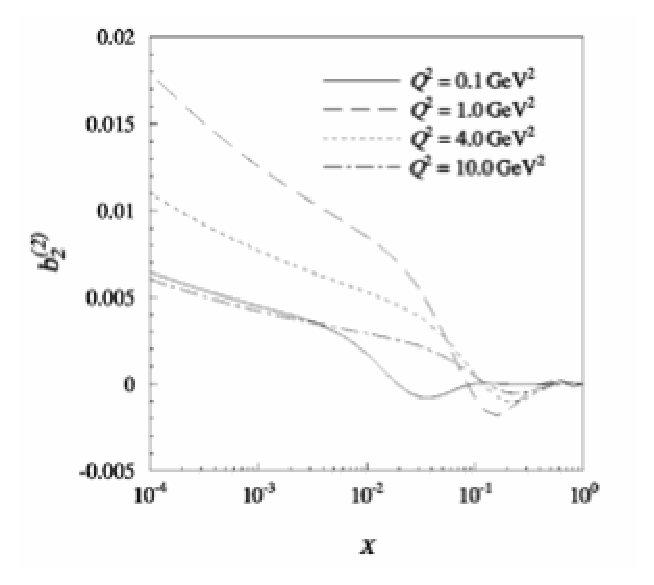
\includegraphics[width=0.5\textwidth]{figs/bora_jaffe_fig3.eps}
%\caption{\label{b2_bora} Double-scattering contribution $b_2^{(2)}(x,Q^2)$ in 
%function of $x$~\cite{Bora:1997pi} (where $2 x b_1 = b_2 = b_2^{(1)}+b_2^{(2)}$).}
%\end{center}
%\end{figure}

\subsubsection{The Close-Kumano Sum Rule}
Following the formalism from the parton model in~\cite{Hoodbhoy:1988am}, Close and 
Kumano ~\cite{Close:1990zw} related the tensor structure function $b_1$ to the electric quadrupole 
form factor of the spin-1 target through a sum rule:
\begin{eqnarray}
\int_0^1 dx~b_1(x)  & = &  - \frac{5}{12 M^2} \lim_{t \rightarrow 0}~t~F_Q(t) 
                           + \frac{1}{9} \Big(\delta Q + \delta \bar{Q}\Big)_s \nonumber \\
                    & = & \frac{1}{9} \Big(\delta Q + \delta \bar{Q}\Big)_s  = 0 \nonumber \\
\label{cksum}
\end{eqnarray}
The sum rule is satisfied in the case of an unpolarized sea. However, the authors emphasize
that in nucleon-only models the integral of $b_1$ is not sensitive to the 
tensor-polarization of the sea, and consequently the sum rule is always true, even when the 
deuteron is in a $D$-state.

Recently, Kumano~\cite{Kumano:2010vz} estimated from an analysis of HERMES data~\cite{Airapetian:2005cb}
that a non-negligible tensor polarization of the sea is necessary to reproduce the trend of
the data. However, this conclusion has to be considered with caution due to the large
$Q^2$ coverage of each HERMES data point (see Fig.~\ref{HERMES_KIN}), and the assumption that 
the sum rule is satisfy for valence quarks.


%



\subsection{Comments from Theorists}
%
During the preparation of this letter, we contacted several theorists 
to gauge interest in a precision measurement of $b_1$.  The response was uniformly positive.  We 
provide some of their feedback for context.
%
%\vspace{0.5cm}
%{\bf S. Kumano (KEK and Tsukuba U.):}
%\vspace{0.5cm}
%{\bf M. Strikman (Penn. State U.) and M. Sargsian (FIU):}
%

\vspace{0.5cm}
``{\it The tensor structure of the deuteron can be investigated in the deep
inelastic region by measuring the structure function $b_1$, which
should shed light on a new aspect of tensor-structure studies in
terms of quark degrees of freedom instead of hadronic ones.
There is a conventional approach for theoretically calculating $b_1$
by quark distribution functions convoluted with nucleon momentum
distributions in the deuteron including the $D$-state admixture.
According to our experience on the nucleon-spin issue, such
a conventional approach for high-energy spin physics would not work.
In particular, it is known that $b_1$ is sensitive to dynamical aspects
of constituents with angular momenta. Measurements of $b_1$ could open
a new field of spin physics because this kind of spin physics has not
been explored anywhere else. Only experimental information came from
the HERMES collaboration; however, their data are not accurate enough
to find $x$ dependence of $b_1$ especially at large $x$. It is
an unique opportunity at JLab to develop this new field of spin physics.}''
\begin{flushright}{\bf S. Kumano (KEK and Tsukuba U.)}\end{flushright}

\vspace{0.5cm}
``{\it I'm glad to hear that $b_1$ is not forgotten in all the excitement about other spin dependent 
effects...
%I don't have much to add to the existing discussion of $b_1$ in the literature. 
%If I remember correctly, 
The hard thing is to distinguish a non-trivial contribution to $b_1$ (eg. 
from 6 quark correlations in the deuteron) from the contribution from the deuteron d-wave.}''
%I 
%also remember a debate about a double scattering contribution.  I wrote a paper on that subject 
%with an Indian visitor to the CTP.  I believe our work was a follow-on to work by Nikolaev and 
%Schafer~\cite{Nikolaev:1996jy}.  I think these papers suggested large contributions to $b_1$ at 
%low x and low $Q^2$.}''
\begin{flushright}{\bf R. Jaffe (MIT)}\end{flushright}

\vspace{0.5cm}
``{\it I am particularly interested in signatures of novel QCD effects in the deuteron. The tensor 
charge could be sensitive to hidden color (non-nucleonic) degrees of freedom at large $x$. It is
also interesting that antishadowing in DIS in nuclei is not universal but depends on the quark 
flavor and spin. One can use counting rules from PQCD to predict the $x \to 1$ dependence of the 
tensor structure function.}''
\begin{flushright}{\bf S. Brodsky (SLAC)}\end{flushright}
 
\vspace{0.5cm}
``{\it I am certainly interested in the experimental development to find the novel
QCD phenomena from the hidden color component of deuteron.}''
\begin{flushright}{\bf Chueng-Ryong Ji (SLAC)}\end{flushright}




\section{The Proposed Experiment}
\begin{figure}
\begin{center}
\includegraphics[width=0.5\textwidth]{figs/plots0705/cov_split_hallC.eps}
\caption{\label{kincov} Kinematic coverage for 11 GeV beam in Hall C using the HMS and SHMS.  A cut will be applied for $W\ge$\WMIN GeV.}
\end{center}
\end{figure}

\label{EXP}
We will measure the leading twist tensor structure
function $b_1$ and tensor asymmetry $A_{zz}$ 
for $\XMIN<x<\XMAX$, $\QMIN<Q^2<\QMAX$ GeV$^2$ and $W \ge \WMIN$ GeV. ~Fig.~\ref{kincov} 
shows the kinematic coverage available at JLab utilizing an 11 GeV beam, 
and the Hall C HMS and SHMS spectrometers at forward angle.


The polarized \TARGET target is discussed in section~\ref{POLTARGSEC}.  
The vector polarization, packing fraction and
dilution factor used in the estimate of the rates are \PZ\%, \PF and \DF respectively. With an incident
electron beam current of \CURRENT nA, the
expected deuteron luminosity is $2\times 10^{35}$ / cm$^2\cdot$s$^1$. The momentum bite and the acceptance
were assumed to be $\Delta P = \pm 8\%$ and $\Delta\Omega = 6.5$ msr for the HMS, and $\Delta P= ^{+20\%}_{-8\%}$ 
%$-8<\Delta P <+20\%$
and $\Delta\Omega =4.4$ msr for the SHMS. 
%
For the choice of the kinematics,
special attention was taken onto the angular and momentum limits of the spectrometers: for the
HMS, $10.5^{\circ} \le \theta \le 85^{\circ}$ and $1 \le P_0 \le 7.3$ GeV/c, and for the SHMS,
$5.5^{\circ} \le \theta \le 40^{\circ}$ and $2 \le P_0 \le 11$ GeV/c. In addition, the
opening angle between the spectrometers is physically constrained to be larger than 17.5$^{\circ}$.
The invariant mass $W$ was kept to $W \ge \WMIN$ GeV for all settings.
The projected 
uncertainties for $b_1$ and $A_{zz}$
are summarized in Table~\ref{RATES} and displayed in
Fig.~\ref{PROJ}.  

A
total of \production_days days of beam time is requested for production data, with an additional \overhead_days days of expected overhead.


\begin{figure}
\begin{center}
\includegraphics[width=0.45\textwidth]{figs/plots0705/b1_proj_newmiller_lin.eps}
\hspace{0.5cm}
\includegraphics[width=0.45\textwidth]{figs/plots0705/Azz_proj_lin.eps}
\caption{\label{PROJ}
{\bf Left: }
Projected precision of the tensor structure function $b_1$  with \production_days days of beam time.
{\bf Right:} Corresponding projected precision of the tensor asymmetry $A_{zz}$. 
The black band
represents the systematic uncertainty.
Also shown are the HERMES data~\cite{Airapetian:2005cb}, and the calculations from Kumano~\cite{Kumano:2010vz}, Miller~\cite{Miller:1989nc,Miller_tmp}, and Sargsian~\cite{MISAK}.
}
\end{center}
\end{figure}
%


\begin{table}
\begin{center}
\begin{tabular}{c|ccc|cc|c|cc|cc|c}
& $\overline{x}$  & $\overline{Q^2}$      &  $\overline{W}$  &    $P_0$    &    $\theta$  &  Rates & $A_{zz}$ & $\delta A_{zz}^{stat}$    & $b_1$  & $\delta b_1^{stat}$ & time   \\
&  ~     & (GeV$^2$)  & (GeV) & (GeV)  &     (deg.)  &   (kHz)  & \multicolumn{2}{|c|}{$\times 10^{-2}$} &  \multicolumn{2}{|c|}{$\times 10^{-2}$}    & (days) \\
%\multicolumn{2}{|c|}{$\times 10^{-2}$}
\hline\hline
SHMS & 0.30&  1.5&  2.11&  8.46&     7.3&    0.48&   0.48&   0.11&  -0.33&   0.072&   15.7 \\
SHMS & 0.40&  2.2&  2.07&  8.20&     9.0&    0.14&   0.99&   0.22&  -0.38&   0.083&   12.5 \\
HMS  & 0.50&  3.5&  2.11&  7.30&    12.2&    0.03&   1.40 &   0.34&  -0.25&   0.062&   28.1 \\  

\hline\hline
\end{tabular}
\caption{\label{RATES}Summary of the kinematics and physics rates using Hall C  spectrometers.}
\end{center}
\end{table}


\subsection{Experimental Method}
\setcounter{footnote}{2}
Following Ref.~\cite{Hoodbhoy:1988am},  we will extract $b_1(x)$ from
%the asymmetry $A_{zz}$ by taking 
the difference of parallel and perpendicular polarized target cross sections, 
with an unpolarized\footnote{Polarized beam is not required for this experiment, but would enable a simultaneous measurement of $g_1$.  The
tensor structure function $b_1$ can then be isolated by averaging the results of data with beam polarized parallel and anti-parallel.  Any contribution from residual vector polarization can be eliminated by grouping together two sets of data of opposing beam helicity.  False asymmetries will be monitored in a similar fashion by periodically flipping the target spin direction.} incident electron beam.  
The polarized cross sections\footnote{For simplicity, we will use $\sigma_{\parallel}$ for $\frac{d\sigma_{\parallel}^H}{dxdy}$ and $\sigma_{\perp}$ for $\frac{d\sigma_{\perp}^H}{dxdy}$.} 
%$d^2\sigma_{\parallel}/d\Omega dE'$ and $d^2\sigma_{\perp}/d\Omega dE'$
can be extracted from data collected by scattering an unpolarized electron beam off a spin-1 target
polarized longitudinally and perpendicularly to the electron beam direction.
%

For this configuration, it can be shown that:
%\begin{eqnarray}
%\frac{\frac{d^2\sigma_{\parallel}}{d\Omega dE'} - \frac{d^2\sigma_{\perp}}{d\Omega dE'}}
%{\frac{d^2\sigma_{\parallel}}{d\Omega dE'} + 2 \frac{d^2\sigma_{\perp}}{d\Omega dE'}} = 
%- \frac{1}{2} (1 - \frac{3}{2} H^2) A_{zz},
%\label{para-perp}
%\end{eqnarray}
%
%where $H^2=(P+2)/3$, with $P$ the deuteron vector polarization.
\begin{eqnarray}
 \sigma_{\perp} - \sigma_{\parallel} = \frac{K}{6} (2 P_z^{\parallel} + P_z^{\perp}) x b_1
\label{MAIN}
\end{eqnarray}
where $P_z^{\parallel}$ and $P_z^{\perp}$ are the vector polarization achieved in the longitudinal and transverse configurations respectively. 
%
The tensor asymmetry can then be extracted from the structure function $b_1$ via:
\begin{eqnarray}
\label{STUFF}
A_{zz} = -\frac{2}{3} \frac{b_1}{F_1} 
\label{Azz}
\end{eqnarray}
The time necessary to achieve the desired precision $\delta b_1$ is:
\begin{eqnarray}
T = \frac{N}{R_D} = \frac{2}{\epsilon^2 R_D (\delta b_1 / b_1)^2}
\label{none}
\end{eqnarray}
%
where $R_D$ is the deuteron rate, which is estimated from Ref.~\cite{Martin:2009iq}, and $\epsilon$ is given  by Eq.~\ref{EPSILON}. 
Full details of the statistical error calculation are provided in Appendix~\ref{APPERR}, for reference.


%From Eq.~\ref{para-perp}, the beam time needed to achieve an absolute uncertainty 
%of $\delta A_{zz}$ can be deduced as:
%\begin{eqnarray}
%T = \frac{32}{9 P_{z}^2} \frac{1}{R_D~f~(P_{zz}~\delta A_{zz})^2}
%\label{time-eq2}
%\end{eqnarray}
%
%where $R_D$ is the deuteron rate, $f$ the dilution factor and $P_{zz}$ the tensor polarization.



\subsubsection{Systematic Uncertainties}
Table~\ref{sys} summarizes the systematic error estimate for the cross section measurement.
The unpolarized structure function
$F_1$ is used to evaluate $A_{zz}$ from the measured $b_1$  using Eq.~\ref{STUFF}.   This contributes an additional 5\% relative, which raises the total systematic for $A_{zz}$ to 10.6\%.

%\begin{table}
%\begin{center}
%\begin{tabular}{l|c}\hline\hline
%Item                         & Systematic \\
%\hline
%Polarimetry                  &   8\%   \\
%Dilution/packing fraction    &   5\%   \\
%Radiative corrections        &   5\%   \\
%%F$_1$ structure function     &   5\%   \\
%Computer deadtime            &  0.5\%  \\
%Charge measurement           &  0.5\%  \\
%Energy measurement           &  0.05\% \\
%\hline
%Total  &  10.7\%   \\
%\hline
%\end{tabular}
%\caption{\label{sys}Relative systematic uncertainties for $A_{zz}$.  }
%\end{center}
%\end{table}

\begin{table}
\begin{center}
  \begin{tabular}{ll} \hline\hline
 Source    &  (\%) \\
  \hline \hline
   Target Polarization                  & 5.0     \\
   Dilution/Packing fraction            & 5.0      \\
   Radiative Corrections                & 4.0     \\
   Acceptance                           & 4.0      \\
   Charge determination      & $\le$1      \\
   VDC efficiency            & $\le$1      \\
   PID detector efficiencies & $\le$1 \\
   Software cut efficiency   & $\le$1 \\
   Energy                    & 0.5      \\
 \hline\hline
    Total                    & 9.3  \\
 %\hline
 \end{tabular}
\caption{\label{sys} Major contributions to the cross section systematic.}
 \end{center}
\end{table}



%\begin{table}
%\begin{center}
%\begin{tabular}{c|ccc}\hline\hline
%     ~                 &  Time   & Number &   Total Time \\
%     ~                 &  (hrs)  &   ~    &    (hrs)     \\
%\hline
%Elastic calibration                &    48.0    &   1    &     48.0     \\
%Target dilution measurement               &    8.0    &   1    &     8.0      \\
%Configuration changes   &   16    &   4    &     64.0     \\
%Beam Energy measurement      &   2.0   &   2    &     4.0      \\
%BCM calibration        &   1.0   &   2    &     2.0      \\
%Target Annealing       &   2.5   &   4    &     10.0     \\
%Target Material Change &   4.0   &   4    &     16.0     \\
%\hline\hline
%\end{tabular}
%\caption{\label{OVHEAD}Summary of the Overhead.}
%\end{center}
%\end{table}


\begin{table}
\begin{center}
  \begin{tabular}{lrrr} \hline\hline
 Overhead & Number&Time Per (hr)&(hr)\\
\hline
Target anneal             &   30&       2.0&      60.0\\
Target field rotation     &    3&       12.0&      36.0\\
Beamline survey           &    2&       8.0&      16.0\\
Target material change    &    5&       8.0&      40.0\\
Target T.E.               &   16&       4.0&      64.0\\
Packing Fraction          &    6&       2.0&     12.0\\
\hline
%Pass change              &    0&       4.0&       0.0\\
Linac change              &    2&       8.0&      16.0\\
Momentum/angle change     &    1&       2.0&       2.0\\
Moller measurement        &    6&       2.0&       12.0\\
Optics                    &    3&       4.0&      12.0\\
Arc Energy Meas.          &    3&       2.0&       6.0\\
BCM calibration           &    2&       2.0&      8.0\\
\hline
                          &     &          &        \overhead_days days  \\
\hline
 \end{tabular}

 \end{center}

  \caption{\label{OVERHEAD} Major contributions to the overhead.}
\end{table}


%\subsection{Alternate Methodology}
%
%In addition to the experimental approach considered in this proposal, we 
% have two other options which we will explore further in preparation for a full proposal: 
%\begin{enumerate}
% \item measuring the tensor structure function $b_1$ with a longitudinally polarized target
%using the cross section method suggested in Ref.~\cite{Hoodbhoy:1988am};
% \item measuring the tensor asymmetry $A_{zz}$ using the HERMES method~\cite{Riedl:2005jq}, 
%with only a longitudinally polarized target.
%\end{enumerate}
%We are also exploring other forms of accessing $A_{zz}$ that don't rely on $A_2^d$ 
%being negligible, like HERMES assumed.




\subsubsection{Overhead}
%
Table~\ref{OVERHEAD} summarizes the expected overhead, which sums to \overhead_days days.
%In order to calibrate the target polarimetry, elastic scattering measurements will be performed at %an 
%incident energy of 2.2 GeV. 
Measurements
of the dilution from the unpolarized materials contained in the target, and of the packing fraction due to
the granular composition of the target material will be performed with a carbon target.
Target annealing will be performed approximately once per day, and target material changes will be performed slightly more than  once a week.
Configuration changes include rotation of the magnetic field of the target from parallel to perpendicular and vice versa.


%\subsection{Background}
%The pion background has not been estimated yet for this measurement, but should be comparable to other
%proposed DIS measurements with HMS and SHMS. A careful study of the background will be performed in a full
%proposal.

%%\subsection{Beamline Instrumentation}

%\subsection{Beamline Instrumentation}
%\subsubsection{Beam Current and Beam Charge Monitor}
%Beam currents less than 100 nA are typically used with the polarized target in order
%to limit depolarizing effects and large variations in the density.  All three experimental halls 
%are instrumented (or will soon be) with appropriate 

%Standard BCM cavities have a linearity good to 0.2\% for currents ranging from 
%180 down to 1 uA. 
%High accuracy at even lower currents will be possible due to ongoing upgrades,
%which will be complete before this experiment might be scheduled.
%In addition, experiment E05-004\cite{eDprop} has just recently  commissioned a tungsten 
%beam calorimeter, in order to have a good calibration for $I<3 \mu A$.
%Preliminary results show an absolute calibration of the Hall A BCM
%with 1\% accuracy for currents ranging from 3 $\mu A$ down to 0.5$\mu A$.
%The calorimeter will be located just after the first BPM and before the first dipole
%(see Fig.~\ref{beamline}).
%In the worst-case scenario, the tungsten calorimeter will allow at least 
%2\% accuracy~\cite{ARNE} on the charge determination all the way down to 50 nA.
%
%\subsubsection{Beam Polarimetry}
%We will utilize the Moeller polarimeter as part of the standard Hall X equipment. 
%During operation, 
%0.3 to 0.5 $\mu A$ of current are incident on  a foil of
%iron polarized by a magnetic field.
%The expected systematic uncertainty~\cite{Alcorn:2004sb} of the Moeller
%measurement is 3.5\% or better. 
%Moeller runs will be scheduled at least once per energy change.


%The Compton polarimeter normally is used for a continuous non-invasive
%beam polarization monitor.  However, it is not very well suited to run
%at low energy or low current.
%To provide a cross check of the Moller polarimeter, we may dedicate some
%high current beam time (without polarized target) specifically for Compton
%polarimeter measurements.





%\subsection{The Spectrometers}
% 
%\subsubsection{Detector Stack }
%The standard detector stack will be used for detecting electrons. We will require the 
%usual VDC,
%scintillators S1 and S2, the gas Cerenkov and
%pion rejector/shower counter for particle identification.
%Performance of the spectrometers are well known 

%\subsubsection{Optics}
%A study of the change of the optics coming from the target field was done by xxxx.



%\subsubsection{Data Acquisition}
%We will utilize the standard Hall X data acquisition (DAQ) system which is based on Fastbus 
%1877 TDC and Fastbus 1881 ADC. 
%The DAQ will be run in two single arm mode which allows up to 4
%KHz rate of data for each arm.  


%\end{document}
%% add GEn review by J.H Mitchell
%%http://galileo.phys.virginia.edu/~dbd/JHM_beamline.pdf





\subsection{Polarized Target}
\label{POLTARGSEC}
This experiment will require the installation of the
JLab/UVa polarized target operated in longitudinal and also transverse mode.  Transverse polarization requires  operation of an upstream chicane to ensure proper transport through the target magnetic field.  The target is typically operated with a specialized slow raster, and beamline instrumentation capable of characterizing the low current 50-100 nA beam.
All of these requirements have been met previously in Hall C.
%, and will be soon implemented also in Hall A for the E08-027/E08-007 run in 2011. 
%
The polarized target (see Fig.~\ref{fig:target}), 
has been successfully used in experiments E143, E155, and E155x at SLAC, and E93-026, E01-006 and E07-003 at JLab. The same target will be utilized in experiments E08-027 and E08-007 in late 2011. 
A similar target was used in Hall B for the EG1,EG4 and DVCS experiments, although Hall B does
not at present have the facilities necessary to operate a transversely polarized target with an electron beam.

The target is in the process of undergoing significant renovation and improvement~\cite{CKEITH}.  The superconducting coils were refurbished by Oxford instruments.  A new 1 K refrigerator and target insert were designed and constructed by the JLab target group.  The cryogenic pumping system has been overhauled.  In particular, the older Alcatel 2060H rotary vane pumps have been replaced with new Pfeiffer DU065 magnetically coupled rotary vane pumps, and the pump controls are being refurbished. The target motion system has been rebuilt from scratch. And now, the magnet and vacuum jacket rotate independently of the refrigerator and target insert, which simplifies rotation from parallel to perpendicular magnetic field orientations.

%
\begin{figure}
\centering
\includegraphics[width=5.0in,clip]{figs/targnew.eps} %target_gimp.eps}
\caption{Cross section view of the JLab/UVa polarized target. Figure courtesy of C. Keith.  \label{fig:target}}
\end{figure}


%\begin{figure}
%\centering
%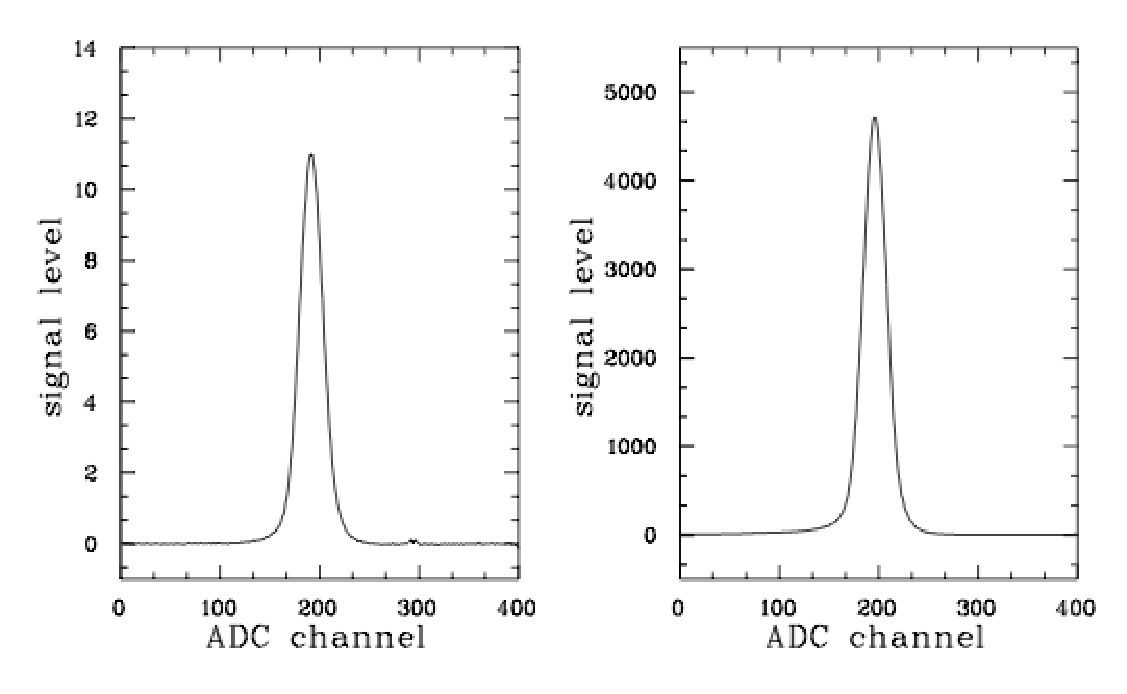
\includegraphics[width=4.5in,clip]{figs/liD.eps}
%\caption{\label{fig:LID} Typical Deuteron thermal equilibrium (TE) and enhanced signals in $^6$LiD.  The left plot shows a typical deuteron TE and the right shows an enhanced deuteron NMR signal.  Note its clean undistorted shape unlike for $^{15}ND_3$.  Also, note the scale difference between the TE and enhanced signals.
%{\it Reproduced from Ref.~\cite{ALTOBIAS}}.}
%\end{figure}

\begin{figure}
\centering
\includegraphics[width=0.5\textwidth]{figs/tensor_pol3.eps}
\caption{{\bf Top}: NMR signal for ND$_3$ with a vector polarization of approximately 50\% from the GeN experiment.  The average polarization in beam for that experiment was 35\%. 
{\bf Bottom}: Relationship between vector and tensor polarization in equilibrium, and 
neglecting the small quadrupole interaction.  \label{fig:tensorpol}}
\end{figure}

\begin{figure}
\centering
\includegraphics[width=3.0in,clip]{figs/gen.eps} %target_gimp.eps}
\caption{Performance of the ND$_3$ target during the GeN experiment.  \label{fig:gen}}
\end{figure}


The target operates on the principle of Dynamic Nuclear Polarization, to
enhance the low temperature (1 K), high magnetic field (5 T) polarization of solid
materials  by microwave pumping.
The polarized target assembly contains several target cells of 3.0 cm length
that can be  selected individually by remote control to be located in the uniform field
region of a superconducting Helmholtz pair. The permeable target cells are
immersed in a  vessel filled with liquid Helium and maintained at 1 K by use of a
high power evaporation refrigerator.
The coils have a 50$^\circ$ conical shaped aperture along the beam axis
which allow for unobstructed forward scattering.
%34$^\circ$ wedge shaped aperture along the vertically oriented midplane.

The target material is exposed to microwaves
to drive the hyperfine transition which  aligns the nucleon spins. 
 The heating of the target by the beam causes a drop of a few percent in
the polarization, and the polarization slowly decreases with time due to radiation
damage. Most of the radiation damage can be repaired by periodically annealing the target,
until the accumulated dose reached is greater than about 
%$ 17\times 10^{15}$ e$^-$/cm$^2$, 
 $0.5\times 10^{17}$ e$^-$/cm$^2$,
at
which time the target material needs to be replaced. 
%The luminosity of the polarized 
%material in the uniform field region is approximately $85\times 10^{33}$ cm$^{-2}$ Hz.

\subsubsection{Polarization Analysis} 
%Eq.~\ref{TENSORVECTOR} allows calculation of a target's tensor polarization once the vector polarization has been determined.  
The three Zeeman sublevels of the deuteron system ($m=-1,0,1$) are
shifted unevenly due to the quadrupole interaction~\cite{Meyer:1985dta}. This shift
depends on the angle between the magnetic field and the electrical field gradient, and gives rise to two separate transition
energies. Hence, the unique double peaked response displayed in Fig.~\ref{fig:tensorpol}.
When the system is at thermal equilibrium with the solid lattice, the deuteron polarization is known from:
\begin{eqnarray}
\label{VECT}
P_z = \frac{4+\tanh\frac{\mu B}{2 k T}} {3+\tanh^2\frac{\mu B}{2 k T}    }
\end{eqnarray}
where $\mu$ is the magnetic moment, and $k$ is Boltzmann's constant.  The vector polarization can be determined by comparing
the enhanced signal with that of the TE signal (which has known polarization).  This polarimetry method is typically reliable to about 5\% relative.

Similarly, the tensor polarization is given by: 
\begin{eqnarray}
\label{TENS}
P_{zz} = \frac{4+\tanh^2\frac{\mu B}{2 k T}} {3+\tanh^2\frac{\mu B}{2 k T}    }
\end{eqnarray}

From Eqs.~\ref{VECT} and~\ref{TENS}, we find:
\begin{eqnarray*}
P_{zz}= 2 - \sqrt{4-3 P_z^2}
\end{eqnarray*}


In addition to the TE method, polarizations can be determined by analyzing NMR lineshapes as described in~\cite{Dulya:1997qc} with a typical  7\% relative uncertainty.  At high polarizations, the
intensities of the two transitions differ, and the NMR signal shows an asymmetry R in the
value of the two peaks, as shown in Fig.~\ref{fig:tensorpol}.  The vector polarization is then given by:
\begin{eqnarray}
\label{RVECT}
P_{z} = \frac{R^2-1}{R^2+R+1}
\end{eqnarray}
and the tensor polarization is given by:
\begin{eqnarray}
\label{TVECT}P_{zz} = \frac{R^2-2 R +1}{R^2+R+1}
\end{eqnarray}


%or by comparison of the NMR response to the known thermal equilibrium (TE) polarization with typical 5\% uncertainty.

The DNP technique produces  deuteron vector polarizations of up to 60\%  in ND$_3$ 
and 64\% in LiD~\cite{Bueltmann:1998wq}, which corresponds to tensor polarizations of approximately 30\%.
%Tensor polarizations of 22\% have been achieved in previous experiments~\cite{Meyer:1985dta}
%using standard solid polarized ammonia targets.
The target polarization decays while in beam, so that the average vector polarization can be
expected to be about 35\%, as seen if Fig.~\ref{fig:gen}.

%While it is not necessary for this experiment, it may be possible to directly determine the tensor polarization directly from the analyzing power T$_{20}$


An average polarization of \PZ~ percent enables a significant measurement of $b_1(x)$, as shown in 
Fig.~\ref{PROJ}.  Any improvement to the expected polarization, although not strictly necessary, 
would allow the addition of kinematic points, and/or improved statistical accuracy.
With this in mind, we are pursuing techniques to enhance the tensor polarization by directly stimulating 
transitions to/from the $M_s=0$ state, as discussed in Ref.~\cite{Meyer:1985dta}.  D. Crabb from the UVa group  
had some success in obtaining enhanced tensor polarizations via RF saturation of one of the Zeeman transitions, otherwise known as `hole-burning'.  The method was not pursued due to the
lack of need for tensor polarized targets at the time of the study.  Another method to enhance tensor polarization entails simultaneously pumping the sample with two independent microwave frequencies, 
which requires careful isolation of the respective cavities. We reiterate that the rates in this proposal assume only polarizations that have been demonstrated previously during typical operation at JLab.








\section{Summary}
  
This experiment will require 38 days of beam time in order to perform a 
precision measurement of $b_1^d$ using a longitudinally polarized deuteron 
(LiD) target, together with the Hall A SoLID spectrometer.



%We request xx days in order to perform a precision measurement of $b_1^d$
%using a longitudinally 
%polarized proton (NH$_3$) target, together with the Hall X xxx detector.
%This experiment is fascinating and all PAC members should be fascinated by it.

\clearpage
\appendix
\section{Statistical error calculations of $A_{zz}$ and $b_1^d$}
%%\subsubsection{Statistical error calculations of $A_{zz}$ and $b_1^d$}
\label{APPERR}
Full details of the error calculation can be found in Ref.~\cite{SOLVI}.

From section 6 of Ref.~\cite{Hoodbhoy:1988am},
%Hoodbhoy, Jaffe and Manihar (Nuc. Phys. B312, p571-588, 1989), 
we have:


\begin{eqnarray}
\frac{d\sigma_{\parallel}^H}{dxdy} & = & K \Bigg[x F_1(x) + \Big(\frac{2}{3} - H^2\Big) x b_1(x) \Bigg]\\
\frac{d\sigma_{\perp}^H}{dxdy}    & = & K \Bigg[x F_1(x) - \Big(\frac{1}{3} - \frac{1}{2}H^2\Big) x b_1(x) \Bigg]
\label{xs} 
\end{eqnarray}
%
with $K = \frac{e^4 M E}{2 \pi Q^4} [1+(1-y)^2]$.
%
For simplicity, we use $\sigma_{\parallel}$ for $\frac{d\sigma_{\parallel}^H}{dxdy}$ and $\sigma_{\perp}$ for $\frac{d\sigma_{\perp}^H}{dxdy}$.

%From Jaffe's email, 
We know that $H^2 = (P_z+2)/3$, where $P_z$ is the vector polarization of the target. 
%This is where is my doubt. From the paper and Jaffe's email, they define $H$ as the polarization along the beam. So my understanding is that $P = P_z$ and it is the vector polarization. 
%
And the tensor polarization $P_{zz}$ is related to $P_z$ via Eq.~\ref{TENSORVECTOR}.
%\begin{eqnarray}
%P_{zz} = 2 - \sqrt{4 - 3 P_z^2}
%\label{none} 
%\end{eqnarray}

The tensor asymmetry $A_{zz}$ depends on $b_1$ and $F_1$:
\begin{eqnarray}
\frac{b_1}{F_1} = - \frac{3}{2} A_{zz}
\label{none} 
\end{eqnarray}


Working with the equations of $\sigma_{\parallel}$ and $\sigma_{\perp}$, we can isolate $A_{zz}$ to find: 
\begin{eqnarray}
\frac{\sigma_{\parallel} - \sigma_{\perp}}{\sigma_{\parallel} + 2 \sigma_{\perp}} = \frac{1}{4} P_z A_{zz}
\label{MAIN} 
\end{eqnarray}

Note, that if the vector polarization in the parallel orientation $P_z^\parallel$
differs from the polarization in the perpendicular orientation
$P_z^\perp$, then Eq.~\ref{MAIN} is modified slightly to:
\begin{eqnarray*}
\frac{\sigma_{\parallel} - \sigma_{\perp}}{\kappa\sigma_{\parallel} + 2 \sigma_{\perp}} = \frac{1}{4} P_z^\parallel A_{zz}
\end{eqnarray*}
where $\kappa={P_z^\perp}/{P_z^\parallel}$.   We've assumed $\kappa=1$ for rates calculations.



In order to calculate the statistical error on $A_{zz}$ we start from:
\begin{eqnarray}
(\delta A_{zz})^2 = \Bigg( \frac{\delta A_{zz}}{\delta \sigma_{\parallel}} \Bigg)^2 (\delta \sigma_{\parallel})^2 + \Bigg( \frac{\delta A_{zz}}{\delta \sigma_{\perp}} \Bigg)^2 (\delta \sigma_{\perp})^2
\label{none} 
\end{eqnarray}
and
\begin{eqnarray*}
\frac{\delta A_{zz}}{\delta \sigma_{\parallel}} & = &\frac{4}{P_z} \Bigg[\frac{- (\sigma_{\parallel} - \sigma_{\perp})}{(\sigma_{\parallel} + 2 \sigma_{\perp})^2} + \frac{1}{\sigma_{\parallel} + 2 \sigma_{\perp}} \Bigg] \\
         & = & \frac{4}{P_z} \frac{3 \sigma_{\perp}}{(\sigma_{\parallel} + 2 \sigma_{\perp})^2}
\label{none} 
\end{eqnarray*}


\begin{eqnarray*}
\frac{\delta A_{zz}}{\delta \sigma_{\perp}} & = &\frac{4}{P_z} \Bigg[\frac{- 2 (\sigma_{\parallel} - \sigma_{\perp})}{(\sigma_{\parallel} + 2 \sigma_{\perp})^2} - \frac{1}{\sigma_{\parallel} + 2 \sigma_{\perp}} \Bigg] \\
         & = & \frac{4}{P_z} \frac{-3 \sigma_{\parallel}}{(\sigma_{\parallel} + 2 \sigma_{\perp})^2}
\label{none} 
\end{eqnarray*}
%
to arrive at:
\begin{eqnarray}
(\delta A_{zz})^2 = \Bigg(\frac{4}{P_z}\Bigg)^2 \Bigg[ \frac{9 \sigma_{\perp}^2 \delta \sigma_{\parallel}^2 + 9\sigma_{\parallel}^2 \delta \sigma_{\perp}^2 }{(\sigma_{\parallel} + 2 \sigma_{\perp})^4} \Bigg]
\label{none} 
\end{eqnarray}

The parallel and perpendicular cross sections have the same kinematical weight $K$. Since $b_1$ is very small compared to $F_1$ (or equivalently, $A_{zz}$ is very small), we can make the assumption $\sigma_{\parallel} \approx \sigma_{\perp} \equiv \sigma$ and  $\delta \sigma_{\parallel} \approx  \delta \sigma_{\perp} \equiv \delta \sigma$. 

\begin{eqnarray}
(\delta A_{zz})^2 = \frac{9 \times 16}{P_z^2} \frac{2 \sigma^2 \delta \sigma^2}{(3 \sigma)^4} = \frac{32}{9 P_z^2} \frac{\delta \sigma^2}{\sigma^2}
\label{none} 
\end{eqnarray}

\begin{eqnarray}
\delta A_{zz} = \frac{4 \sqrt{2}}{3 P_z} \frac{\delta \sigma}{\sigma} =  \frac{4 \sqrt{2}}{3 P_z} \frac{1}{\sqrt{N}}
\label{none} 
\end{eqnarray}

We determine $N$ from the unpolarized cross section model~\cite{Martin:2009iq}, which then allows us to calculate the rates and the time.

\begin{eqnarray}
N = \frac{32}{9} \frac{1}{P_z^2 (\delta A_{zz}^{meas})^2}
\label{none} 
\end{eqnarray}

To get the rates as a function of the theoretical tensor asymmetry, we need to apply the dilution factors:
\begin{eqnarray}
A_{zz}^{meas} = f P_{zz} A_{zz}
\label{none} 
\end{eqnarray}

\begin{eqnarray}
N = \frac{32}{9} \frac{1}{P_z^2 (f P_{zz} \delta A_{zz})^2}
\label{none} 
\end{eqnarray}

We need $N/2$ events in parallel and perpendicular kinematics. If we had a pure deuterium target, the time need will be:
\begin{eqnarray}
T = \frac{N}{R_D} = \frac{32}{9} \frac{1}{R_D P_z^2 (f P_{zz} \delta A_{zz})^2}
\label{none} 
\end{eqnarray}

Now the deuterium rates are estimated from the unpolarized deuteron cross section model~\cite{Martin:2009iq} $\sigma_D$:
\begin{eqnarray}
 R_D = \sigma_D~dp~d\Omega~L = \sigma_D~dp~d\Omega~\rho_D~\frac{I}{e}
\label{none} 
\end{eqnarray}
%
with $\rho_D = \rho_{LiD} \cdot f_{LiD} \cdot PF_{LiD}$, where $f_{LiD}$ is the dilution and $PF_{LiD}$ is the packing fraction.





\label{APPERR}
Full details of the error calculation can be found in Ref.~\cite{SOLVI}.
%
From section 6 of Ref.~\cite{Hoodbhoy:1988am},
%Hoodbhoy, Jaffe and Manihar (Nuc. Phys. B312, p571-588, 1989),
we have:

\begin{eqnarray}
\frac{d\sigma_{\parallel}^H}{dxdy} & = & K \Bigg[x F_1(x) + \Big(\frac{2}{3} - H^2\Big) x b_1(x) \Bigg]\\
\frac{d\sigma_{\perp}^H}{dxdy}    & = & K \Bigg[x F_1(x) - \Big(\frac{1}{3} - \frac{1}{2}H^2\Big) x b_1(x) \Bigg]
\label{xs} 
\end{eqnarray}
%
with $K = \frac{e^4 M E}{2 \pi Q^4} [1+(1-y)^2]$.

For simplicity, we will use $\sigma_{\parallel}$ for $\frac{d\sigma_{\parallel}^H}{dxdy}$ and $\sigma_{\perp}$ for $\frac{d\sigma_{\perp}^H}{dxdy}$.


We know that $H^2 = (P+2)/3$, where $P$ is the vector polarization of the target. 
And the tensor polarization $P_{zz}$ is related to $P_z$ via Eq.~\ref{TENSORVECTOR}.

The tensor asymmetry $A_{zz}$ depends on $b_1$ and $F_1$:
\begin{eqnarray}
\frac{b_1}{F_1} = - \frac{3}{2} A_{zz}
\label{none} 
\end{eqnarray}

\subsection{Cross section method}

Working with the equations of $\sigma_{\parallel}$ and $\sigma_{\perp}$, we can isolate $b_{1}$:

\begin{eqnarray}
\sigma_{\parallel} - \sigma_{\perp} = \frac{-K}{6} (2 P_z^{\parallel} + P_z^{\perp}) x b_1
\label{MAIN}
\end{eqnarray}
where $P_z^{\parallel}$ and $P_z^{\perp}$ are the vector polarization achieved in the longitudinal and transverse configurations respectively.
%
%Note, that if the vector polarization in the parallel orientation $P_z^\parallel$
%differs from the polarization in the perpendicular orientation
%$P_z^\perp$, then Eq.~\ref{MAIN} is modified slightly to:
%\begin{eqnarray*}
%\frac{\sigma_{\parallel} - \sigma_{\perp}}{\kappa\sigma_{\parallel} + 2 \sigma_{\perp}} = \frac{1}{4} P_z^\parallel A_{zz}
%\end{eqnarray*}
%where $\kappa={P_z^\perp}/{P_z^\parallel}$.   We've assumed $\kappa=1$ for rates calculations.

\begin{eqnarray}
\frac{\delta b_1}{b_1} = \frac{\sqrt{\delta \sigma_{\perp}^2 + \delta \sigma_{\parallel}^2}}{\sigma_{\perp} - \sigma_{\parallel}} 
\label{none} 
\end{eqnarray}

In the valence region, $b_1 < 0$ which implies $\sigma_{\perp} < \sigma_{\parallel}$. We can define the difference between $\sigma_{\perp}$ and $\sigma_{\parallel}$ as:

\begin{eqnarray}
\sigma_{\parallel} = (1+\epsilon) \sigma_{\perp}
\label{none} 
\end{eqnarray}

It is safe to assume that we will need $\delta \sigma_{\perp} \approx \delta \sigma_{\parallel}$. We obtain:
\begin{eqnarray}
\frac{\delta b_1}{b_1} = - \frac{\sqrt{2}}{\epsilon} \frac{\delta \sigma_{\perp}}{\sigma_{\perp}} 
\label{none} 
\end{eqnarray}

Now to evaluate the time necessary to perform a significant measurement of $b_1$, we need an estimate of the value of $\epsilon$.  So we start from:
\begin{eqnarray}
\sigma_{\parallel} & = & \sigma_{u} (1 - \frac{1}{3} P_z^{\parallel} \frac{b_1}{F_1}) \\
\sigma_{\perp} & = & \sigma_{u} (1 + \frac{1}{6} P_z^{\perp} \frac{b_1}{F_1})
\label{none} 
\end{eqnarray}
%
with $\sigma_u$ the unpolarized cross section.  Which leads to:

\begin{eqnarray}
\epsilon = & \frac{1 - \frac{1}{3} P_z^{\parallel} \frac{b_1}{F_1}}{1 + \frac{1}{6} P_z^{\perp} \frac{b_1}{F_1}}
\label{EPSILON} 
\end{eqnarray}

We use for $b_1^d$ the fit from Kumano~\cite{Kumano:2010vz} and for $F_1^d$ MSTW~\cite{Martin:2009iq} (no EMC effect or smearing included). For $x$-values of 0.30, 0.40 and 0.50, $\epsilon$ is equal to 0.0013, 0.0026 and 0.0037 respectively, assuming $P_z^{\perp} = P_z^{\parallel} = 0.35$

\begin{eqnarray}
\frac{\delta b_1}{b_1} = - \frac{\sqrt{2}}{\epsilon} \frac{1}{\sqrt{N}} 
\label{none} 
\end{eqnarray}

The number of events needed in each parallel and perpendicular kinematics are $N/2$ with:
\begin{eqnarray}
N = \frac{2}{\epsilon^2} \frac{1}{(\delta b_1 / b_1)^2}
\label{none} 
\end{eqnarray}

The time necessary to achieve this statistics is:
\begin{eqnarray}
T = \frac{N}{R_D} = \frac{2}{\epsilon^2 R_D (\delta b_1 / b_1)^2}
\label{none} 
\end{eqnarray}

The deuterium rates are estimated from the unpolarized deuteron cross section~\cite{Martin:2009iq} $\sigma_D$:
%MRST2008:
\begin{eqnarray}
 R_D = \sigma_D~dp~d\Omega~L = \sigma_D~dp~d\Omega~\rho_D~\frac{I}{e}
\label{none} 
\end{eqnarray}
%
with $\rho_D = \rho_{ND3} \cdot f_{ND3} \cdot PF_{ND3}$, where $f_{ND3}$ is the dilution and $PF_{ND3}$ is the packing fraction. To estimate the physics rates, the spectrometer acceptance and momentum bite were reduced to $d\Omega = 6.5$ msr and $dp = \pm$8\% for the HMS and $d\Omega = 4.4$ msr and $dp = ^{+20\%} _{-8\%}$ for SHMS and a cut on $W \ge 1.8$ GeV was required.



%%\section{Asymmetry method}
%
%Working with the equations of $\sigma_{\parallel}$ and $\sigma_{\perp}$, we can isolate $A_{zz}$:
%\begin{eqnarray}
%\frac{\sigma_{\parallel} - \sigma_{\perp}}{\sigma_{\parallel} + 2 \sigma_{\perp}} = \frac{1}{4} P_z A_{zz}
%\label{none} 
%\end{eqnarray}
%
%\vspace{0.5cm}
%\underline{Calculation of $A_{zz}$ statistical error}
%\begin{eqnarray}
%(\delta A_{zz})^2 = \Bigg( \frac{\delta A_{zz}}{\delta \sigma_{\parallel}} \Bigg)^2 (\delta \sigma_{\parallel})^2 + \Bigg( \frac{\delta A_{zz}}{\delta \sigma_{\perp}} \Bigg)^2 (\delta \sigma_{\perp})^2
%\label{none} 
%\end{eqnarray}
%
%\begin{eqnarray}
%\frac{\delta A_{zz}}{\delta \sigma_{\parallel}} & = &\frac{4}{P_z} \Bigg[\frac{- (\sigma_{\parallel} - \sigma_{\perp})}{(\sigma_{\parallel} + 2 \sigma_{\perp})^2} + \frac{1}{\sigma_{\parallel} + 2 \sigma_{\perp}} \Bigg] \\
%         & = & \frac{4}{P_z} \frac{3 \sigma_{\perp}}{(\sigma_{\parallel} + 2 \sigma_{\perp})^2}
%\label{none} 
%\end{eqnarray}
%
%
%\begin{eqnarray}
%\frac{\delta A_{zz}}{\delta \sigma_{\perp}} & = &\frac{4}{P_z} \Bigg[\frac{- 2 (\sigma_{\parallel} - \sigma_{\perp})}{(\sigma_{\parallel} + 2 \sigma_{\perp})^2} - \frac{1}{\sigma_{\parallel} + 2 \sigma_{\perp}} \Bigg] \\
%         & = & \frac{4}{P_z} \frac{-3 \sigma_{\parallel}}{(\sigma_{\parallel} + 2 \sigma_{\perp})^2}
%\label{none} 
%\end{eqnarray}
%
%\begin{eqnarray}
%(\delta A_{zz})^2 = \Bigg(\frac{4}{P_z}\Bigg)^2 \Bigg[ \frac{9 \sigma_{\perp}^2 \delta \sigma_{\parallel}^2 + 9\sigma_{\parallel}^2 \delta \sigma_{\perp}^2 }{(\sigma_{\parallel} + 2 \sigma_{\perp})^4} \Bigg]
%\label{none} 
%\end{eqnarray}
%
%The parallel and perpendicular cross sections have the same kinematical weight $K$. Since $b_1$ is very small compared to $F_1$ (or $A_{zz}$ is very small), we can make the assumption $\sigma_{\parallel} \approx \sigma_{\perp} \equiv \sigma$ and  $\delta \sigma_{\parallel} \approx  \delta \sigma_{\perp} \equiv \delta \sigma$. 
%
%\begin{eqnarray}
%(\delta A_{zz})^2 = \frac{9 \times 16}{P_z^2} \frac{2 \sigma^2 \delta \sigma^2}{(3 \sigma)^4} = \frac{32}{9 P_z^2} \frac{\delta \sigma^2}{\sigma^2}
%\label{none} 
%\end{eqnarray}
%
%\begin{eqnarray}
%\delta A_{zz} = \frac{4 \sqrt{2}}{3 P_z} \frac{\delta \sigma}{\sigma} =  \frac{4 \sqrt{2}}{3 P_z} \frac{1}{\sqrt{N}}
%\label{none} 
%\end{eqnarray}
%
%I get $N$ from the unpolarized cross sections. Then I calculate the rates and the time.
%
%\begin{eqnarray}
%N = \frac{32}{9} \frac{1}{P_z^2 (\delta A_{zz}^{meas})^2}
%\label{none} 
%\end{eqnarray}
%
%To get the rates as a function of the theoretical tensor asymmetry, we need to apply the dilution factors:
%\begin{eqnarray}
%A_{zz}^{meas} = f P_{zz} A_{zz}
%\label{none} 
%\end{eqnarray}
%
%\begin{eqnarray}
%N = \frac{32}{9} \frac{1}{P_z^2 (f P_{zz} \delta A_{zz})^2}
%\label{none} 
%\end{eqnarray}
%
%We need $N/2$ events in parallel and perpendicular kinematics. If I had a pure deuterium target, the time need will be:
%\begin{eqnarray}
%T = \frac{N}{R_D} = \frac{32}{9} \frac{1}{R_D P_z^2 (f P_{zz} \delta A_{zz})^2}
%\label{none} 
%\end{eqnarray}
%
%Now the deuterium rates are estimated from the unpolarized deuteron cross section $\sigma_D$:
%\begin{eqnarray}
% R_D = \sigma_D~dp~d\Omega~L = \sigma_D~dp~d\Omega~\rho_D~\frac{I}{e}
%\label{none} 
%\end{eqnarray}
%
%with $\rho_D = \rho_{LiD} \cdot f_{LiD} \cdot PF_{LiD}$, where $f_{LiD}$ is the dilution and $PF_{LiD}$ is the packing fraction.
%
%
%
%

%  Go to fullpage mode

\topmargin 0pt
\advance \topmargin by -\headheight
\advance \topmargin by -\headsep

\textheight 8.9in

\oddsidemargin 0pt
\evensidemargin \oddsidemargin
\marginparwidth 0.5in

\textwidth 6.5in
\clearpage
%\begin{thebibliography}{99}
%\input{input/bib.tex}
%\end{thebibliography}

 \bibliography{input/tensor_b1}
\end{document}
